\documentclass[11pt, a4paper]{article}

\usepackage{mlt-thesis-2015}

% With Xetex/Luatex this shouldn't be used
%\usepackage[utf8]{inputenc}

\usepackage[english]{babel}
\usepackage{graphicx}
\usepackage{caption}
% \usepackage{subcaption}

\usepackage{setspace}
\usepackage{subfiles} 
\usepackage{hyperref}
\usepackage{booktabs}
\usepackage{comments}
\usepackage{makecell}
\usepackage{amsmath}
\usepackage{subfigure}
%\graphicspath{ {figures/} }

\hypersetup{
colorlinks,
allcolors={blue}
}


\title{Spatial Relations in Emergent Languages}
\subtitle{This is the subtitle}
\author{Dominik Künkele}

\begin{document}

%% ============================================================================
%% Title page
%% ============================================================================
\begin{titlepage}

    \maketitle

    \vfill

    \begingroup
    \renewcommand*{\arraystretch}{1.2}
    \begin{tabular}{l@{\hskip 20mm}l}
        \hline
        Master's Thesis:   & 30 credits                                \\
        Programme:         & Master’s Programme in Language Technology \\
        Level:             & Advanced level                            \\
        Semester and year: & Spring, 2023                              \\
        Supervisor:        & Simon Dobnik                              \\
        Examiner:          & Asad Sayeed                               \\
        Keywords:          & keyword 1, keyword 2, keyword 3
    \end{tabular}
    \endgroup

    \thispagestyle{empty}
\end{titlepage}

%% ============================================================================
%% Abstract
%% ============================================================================
\newpage
\singlespacing
\section*{Abstract}


\thispagestyle{empty}

%% ============================================================================
%% Preface
%% ============================================================================
\newpage
\section*{Preface}



\thispagestyle{empty}

%% ============================================================================
%% Contents
%% ============================================================================
\newpage

\begingroup
\hypersetup{linkcolor=black} % This ensures that ONLY the ToC has black links
\begin{spacing}{0.0}
    \tableofcontents
\end{spacing}
\endgroup

\thispagestyle{empty}

%% ============================================================================
%% Introduction
%% ============================================================================
\newpage
\setcounter{page}{1}

\section{Introduction}
\label{sec:introduction}
Language is a complex system that enables humans to communicate and convey meaning. However, the mere existence of words and grammatical structures is not enough to guarantee effective communication. Without grounding, language remains detached from the physical world, making it difficult for individuals to comprehend and interpret linguistic expressions accurately.
Grounding bridges the gap between abstract linguistic representations and concrete experiences, providing a shared context and reference point for language users \citep{Roy2002,Bisk2020,Bender2020}. By linking language to sensory perceptions, physical experiences, and the situational context, grounding enhances comprehension, facilitates communication.
However, one challenge lies in how arbitrary symbols in language can be connected to real-world objects and concepts and acquire meaning, described as the symbol grounding problem by \citet{Harnad1990}.
Artificial agents can be taught grounding in different ways.
One approach is to show the agent an image of the scene as visual input together with a textual description of what is to be grounded in this scene.
This can be for example a description of the whole scene, certain visible objects or also actions that are happening \citep{Ahrens2022,Ilinykh2022,Lu2017,Mitchell2013}.
By doing this, the agents can learn to identify the same descriptions and symbols for similar visual input.
In other approaches, the agents can learn to ground language in visual input through interaction and dialogue, either with humans or other agents.
Thus, agents might develop certain strategies to ground language efficiently \citep{Dobnik2018a,Dobnik2021,Zarriess2019}.

A central part in many of the ways to learn to ground are referring expressions.
Referring expressions are used to point out a particular subset of entities from a set of similar entities or the surrounding context.
By that, they can take many forms as noun phrases (e.g. 'the large table', 'the second chair from the right'), proper nouns (e.g. 'Francesca', 'the Big Ben') or complete descriptions (e.g. 'the men that are wearing glasses').
When referring to objects, they often include inherent attributes of these objects as their color or shape.
Furthermore, spatial terms play a vital role to refer to and disambiguate objects \citep{Regier1996,  Dobnik2013, Dobnik2021,Ghanimifard2017, Ramisa2015}.

One problem that arises is the question of ambiguity in language and referring expressions.
Natural language is often used in an underspecified way.
Interlocutors rely on pragmatic and semantic context to communicate.
Given for example the following situation:
Two people are in a room with two chairs.
If one person asks for 'a chair', the second person would give him the chair that is closer to him.
In other situations the second person would give him his preferred chair even if it's further away.
The referring expression is the same in both contexts, but refers to two different entities.
The difference lies in the pragmatic context that both interlocutors are aware of.
In case this context is not shared, referring expressions might be misunderstood, because of the underspecification.

Furthermore, the real world is characterized by its continuous nature.
On the other side, natural language is a set of discrete symbols.
In the process of mapping this continuum to the discrete symbols, information is lost, since the whole context of the real world can't be captured by the natural language.
By this, symbols get ambiguous and refer to multiple concepts in the world.
One example are the shades of color \citep{Zaslavsky2018}.
Discrete English terms like 'red', 'green' or 'blue' might refer to an infinite number of colors in the real world.

To deal with this, humans rely on communicative protocols to disambiguate referring expressions.
\citet{Dale1995}, for instance, describe an incremental algorithm how referring expressions are generated.
The goal of the algorithm is to construct referring expressions incrementally, taking into account the salience of different properties and abstracting away from differences in lexical choice.
It works by gradually building up a referring expression based on the properties of the object being referred to.
Hereby, it considers the most salient or distinguishing properties first and then adds additional properties as needed.
This helps to create concise, effective and disambiguous referring expressions.
\cmtDK[inline]{co-reference}

Meaning of symbols and referring expression emerge through dialogue between interlocutors \citep{Wittgenstein1953,Clark1986}.
Moreover, \citet{Wittgenstein1953} introduces the concept of \emph{language games}: small parts of conversation between interlocutors.
In these language games, their context defines which meaning emerges for the referring expressions.
This reasoning was taken up in training artificial agents to learn to refer to entities.
Hereby, agents need to communicate arbitrary symbols to each other in multiple turns to solve a given task.
By solving the task, they assign meaning to these symbols and an artificial language emerges.
This setup allows to control the architecture of the agents, the information the agents receive, how and what they are able to communicate and which goals they are trained on.
By this, their behavior and the emergence of referring expressions can be studied precisely and consistently.
In early research, agents and their communication were studied in the context of robotics and rule-based systems \citep{Steels2009,Roy2002,Kirby2002,Kirby2008}, while in current research, agents are based on deep neural networks \citep{Lazaridou2017,Baroni2020,Baroni2022,Kottur2017}
Furthermore, a focus lies on the nature of the emerged language.
Agents can for instance learn a compositional language that allows them to combine already learned symbols to create new meaning, when presented with a changed environment and unseen situations \citep{Kharitonov2020,Lazaridou2018,Gupta2020}.
Additionally, emergent languages can be learned to encode meaning in efficient ways \citep{Chaabouni2019,Zaslavsky2018}.

% SD: I would turn the order of this around, it would make the motivation clearer. The introduction should also be much longer with linguistic examples and citations of related work (but I see that you want to keep it for later.)
% SD: Our goal is to study referring, how we refer to entities and have we interpret the entities referred to. 
% SD: There is a lot of ambiguity involved as language only maps to the world in an under specified way.  The first problem is that a word may map to several pixels. There is a loss of information/abstraction. The second problem is that referring expressions are under-specified, chair can be any of the 5 chairs. This is to compress information in communication, we say less than we mean. Illustrate both points with examples.
% SD: Instead, humans rely on communicative protocols to disambiguate referring expressions. The Dale and Reiter algorithm and the literature on GRE. Communicative protocols are established through language games, some parts seen to be universal, some parts are negotiated on the fly.
% SD: Artificial language games - describe in more detail what they are and how they are implemented - allow us to study language with8n this communicative setting. 
% SD: In this thesis we look at referring within the context of communicative games to explore both theoretical and practical (computational) limits of grounded referring expressions in interactive setting.
% SD: The novelty of this thesis is that we study referring to entities through language games involving sequences of descriptions.
% SD: Here we need to cite: (1) literature on grounding, connecting language and vision, Harnad, Roy, us, etc. (2) referring expression generation, Dale and Reiter, (4) reference and co- reference (Poesio, us), (5) language games (Wittgenstein) and referring as a collaborative process (Clark, David Lewis), (6) language games (work by Kazakov and Kirby), within robotics (Steels), language games within neural models (Baroni).
% SD: Mathias’ work is also relevant https://era.ed.ac.uk/handle/1842/38727
% DK: TODO

\subsection{Research Questions}
In this thesis, a deeper look is taken into how agents can ground their emerged language in visual input.
The focus hereby lies on referring expressions and how agents are able to generate and understand them.
Multiple experiments are designed in a way that agents need to use referring expressions in their messages that are communicated.
These messages are analyzed with respect to the visual input to answer the two following questions:
\begin{enumerate}
      % \item Are cooperative agents in language games able to generate and understand artificial referring expressions based on visual input?
      \item What are the limits of the agents' architectures and input representations on learning successfully grounding referring expressions through language games?
            % SD: What are the limits of the agent architecture and and input representation on learning successful grounding referring expressions through language games?
            % DK: (done)
            % \item If a language emerges, how similar are the referring expressions to referring expressions that are used in English?
      \item To what degree do emergent referring expressions align with referring expressions in a natural language such as English and what constraints can be imposed on the environment and the agents themselves that languages align?
            % SD: To what degree does the emergent referring expressions align with referring expressions in a natural language such as English what constraints can be imposed on the environment and the agents themselves that languages align?
            % DK: (done)
\end{enumerate}


\subsection{Contribution}
This thesis aims to add three contributions to the field of research.
First, new artificial visual datasets are created, consisting of images, depicting objects and their attribute and spatial relations.
Many existing datasets that are used to study referring expressions that use real images are based on photos taking by humans.
This adds a lot of inherent bias to the dataset, since these photos often focus on similar objects and actions.
Additionally, they require external knowledge about the world and the functions of objects which is not present in the image.
Furthermore, information about the objects and their relations in the image are not present in a structured way.
The datasets that are created in this thesis aim to reduce this bias and provide all information about the scene and objects in the image.
In fact, the artificial creation of the dataset allows controlling precisely bias in each scene.
% SD: We also know the ground truth about the scenes as we know the function that generated them.
% DK: (done)

Secondly, the thesis evaluates these datasets, by training separate models to generate and understand referring expressions, describing objects in the images.
By doing this, it is tested if first the models are able to extract useful visual information that doesn't rely on bias and latent patterns in the textual information in the dataset and secondly shows the impact of different levels of ambiguity in the datasets on the performance of generating and understanding of referring expressions.
% SD: We can control the properties of these datasets and we can introduce as much bias and ambiguity as we see firm in each experiment to compare with the natural datasets.
% DK: (done)

Lastly, the thesis brings the separate tasks of generating and understanding of referring expressions together into one single task.
This process resembles the learning of referring expressions in natural language \citep{Clark1986}.
% SD: Which is how this is done in practice, cf. referring as a collaborative process, the paper by Clark.
% DK: (done)
In language games, one agent needs to extract visual information from an image and generate a referring expression that is sent to the second agent.
The second agent on the other hand needs to understand this referring expressions and combine it with its visual input.
Only if both of these subtasks succeed, a new artificial language can emerge and the overall task can be solved.
The emerging language is then analyzed to understand, how the artificial referring expressions are built up and compare to natural language.

\subsection{Scope}
The focus of this thesis is the study of referring expressions.
Referring expressions can hereby be based on inherent attributes of objects, as well as their spatial relations towards other objects.
In the present study, only the relations of the inherent attributes are studied.
% SD: What are those?
% DK: (done)
Spatial relations add another level of complexity and may be studied in future work.
% SD: What kind of complexity?
% DK: (done)
Furthermore, the emerged language will be interpreted by comparing it to referring expressions in natural language.
This analysis focuses on the emerged meaning of symbols and if they align with natural language.
A deeper study of its compositionality or complexity is out of scope.
% SD: Leave for the last chapter, limitations and future work.
% DK: (done)


%% TODO:
% write motivation
% proofread subsection 3
% etc

%% ALREADY DONE:
% write xyz
% fixed bibtex
% etc

%% You can add and edit these comments as you see fit for the other sections, or use some other tool

\newpage

\section{Background and Related Work}
\label{sec:background}
% subsections are \subsection{title}
%% subssubsections are \subsubsection{title}
%% numbering will work automatically 

\subsection{Distributional Hypothesis}

The Distributional Hypothesis is the theory that drives the current... 

In \autoref{subsec:lsc}, we discuss how it is applied to the subfield of ...

\subsection{Lexical Semantic Change (LSC)}
\label{subsec:lsc}

LSC detection through computational methods still...
\newpage

\section{Methodology and Frameworks}
\label{sec:methodology}

\subsection{CLEVR framework}
The basis for my datasets is the Visual Question Answering (VQA) framework CLEVR \citep{Johnson2017a}.
This framework provides code to generate configurable VQA datasets that are split in two parts: a collection of images, and a set of questions and answers that refer and describe each image.
Many of the existing VQA datasets come with two problems.
First, they include many biases, such as biases in the base images and biases in the linguistic properties of the questions and answers.
A relatively high number of images of dogs in a dataset, might for instance bias a classifier model towards classifying dogs most of the time.
On the other hand, repeating patterns in the questions and answers might also be exploited by a model, without extracting the needed information from the image.
For these reasons the CLEVR framework aims to reduce the biases as much as possible in both images and questions and answers as well as precisely control the remaining biases to explore their limits.
% SD: Rather, being an artificial dataset, it allows us to precisely control the bias and therefore explore its limits.
% DK: (added; done)
Secondly, datasets may come with only a limited amount of annotations and information about the state in an image.
The CLEVR dataset uses artificially rendered 3D-scenes.
By doing so, all information about for instance the location of objects or their relations to each other can be later used in training models or analyzing their results.
Furthermore, it allows making predictions about different effects of varying contexts.
% SD: We know the ground truth function that generated the scenes and hence we can also make predictions about different effects of contexts.
% DK: (added; done)

For this thesis, the CLEVR framework will be extended to have more control over the generation of the images.
With this extension, several datasets are created.
The extensions are described in Chapter \ref{sec:creation-dataset}.
Hereby, only the images and their ground truth properties are interesting for the present study of referring expressions.
% SD: We will use the code to generate a new dataset of scenes and descriptions with the properties we want to study.
% SD: You are not just taking their dataset but you are taking the framework and you are applying it on a new task, to generate a new dataset(s) with carefully controlled properties. The CLEVR framework is suitable for this because…
% DK: made clearer, what is done in the thesis, and what described in which chapter (done)
The questions and answers won't be used.
In the following section the image generation of the original CLEVR framework is described.
The visual part contains images of 3D-generated scenes depicting different kinds of simple objects.
Each of these objects is made up of a different combination of attributes, such as \emph{shape}, \emph{color}, \emph{size} and \emph{material}.
The possible values of these attributes are listed in Table \ref{tab:clevr-attributes}.
% SD: Reference to GitHub, also perhaps in the following text when you describe your own code, it would be good to include a reference to the code as you go along.
% DK: this only describes the original framework, my extension is in the next chapter with reference (done)
Three to ten objects are placed in random locations into the scene and assigned with random attributes.
To enhance realism and reduce ambiguity, objects are placed in a way that they do not intersect and have a certain distance from each other
Furthermore, it is made sure that every object is almost completely visible.
The position of the light and the camera are slightly jittered for each image to add noise reduce recurring patterns.
Since the objects are part of 3-d scenes, they may appear differently for each image, because of different lighting and shadows, distances to the camera and rotations.
This noise approximates the real world and natural environment, and makes it harder to learn for models compared to relatively noise-free projections on a 2-d plane.
Figure \ref{fig:clevr-example} shows an example of a generated image in the CLEVR dataset.

\begin{table}[ht]
    \centering
    \begin{tabular}{cccc}
        \toprule
        \textbf{ shape } & \textbf{ color } & \textbf{ size } & \textbf{ material } \\
        cube             & gray             & small           & rubber              \\
        sphere           & red              & large           & metal               \\
        cylinder         & blue                                                     \\
                         & green                                                    \\
                         & brown                                                    \\
                         & purple                                                   \\
                         & cyan                                                     \\
                         & yellow                                                   \\
        \bottomrule
    \end{tabular}
    \caption{Attributes of objects in the CLEVR dataset}
    \label{tab:clevr-attributes}
\end{table}

\begin{figure}[ht]
    \centering
    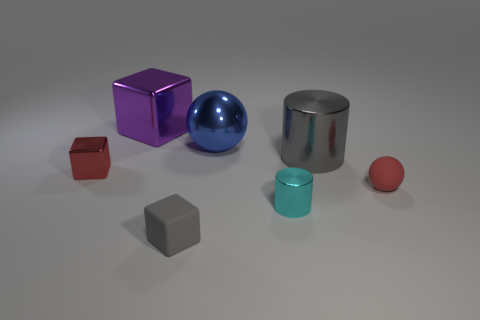
\includegraphics[width=.8\linewidth]{figures/CLEVR_example.png}
    \caption{Example of a generated image in the CLEVR dataset}
    \label{fig:clevr-example}
    % SD: Give also example of ground truth features that were used to generate this, i.e. objects and attributes.
    % DK: TODO
\end{figure}

Furthermore, the dataset contains information about each scene.
This includes all selected attributes for each object as well as the exact position of the centers of all the objects, both 3D-coordinates in the 3D scene and 2D-coordinates in the final rendered image.
In addition, simple spatial relations (in front of, behind, left, right) between the objects are calculated and stored.
% SD: For this, functions from the existing code are used, right?
% DK: exactly. Here, it is only described, what is part of the original CLEVR dataset (done)
These are simply based on the 3D-coordinates of the objects in relation to the position of the camera.

\subsection{Feature extractors}
\cmtDK[inline]{preprocessing}
In computer vision tasks, machines need to analyze images and extract information from them.
To do this, machines often rely on feature extractors.
Features are important parts or patterns in an image, which can have different levels of abstractions.
They can for example be low-level features, as geometric information about lines and edges in an image, or also very abstract information about whole objects.
Traditional approaches involve extracting key points and descriptors from an image and using them to represent the image \citep{Harris1988,Lowe1999,Bay2006}.
More recently, convolutional neural networks (CNN) became popular due to their ability to learn complex features automatically from raw image data.
These are also used in this thesis as a first layer to extract important information from the image. Hereby, two different architectures are tested.
\cmtDK[inline]{explain advantage of CNN}

First, we use the VGG19 \citep{Simonyan2015} which is an architecture based on many convolutional layers.
Using 16-19 convolutional layers with small convolution filters helps the model to solve localization and classification tasks on the training dataset, but also enables is to generalize onto other datasets.
After the convolutional layers, the data is passed first through an average pooling layer which outputs 512x7x7 dimensions.
Next follow three linear layers with \emph{ReLU} non-linearities in between.
After flattening the input, these classification layers output 4069, 4069 and 1000 dimensions respectively.

Secondly, we include the ResNet-101 \citep{He2016}.
This architecture tries to overcome the degradation of very deep networks, where the accuracy rapidly drops after it gets saturated.
This is done using residual blocks.
A residual block consists of two or three convolutional layers and a residual connection, also known as a shortcut connection.
The residual connection allows the input to be added directly to the output of the block, allowing the network to learn the residual function with respect to the input.
This approach enables the network to better preserve information from earlier layers and avoid the problem of information loss that can occur in very deep networks.
There are four blocks that output 256x56x56, 512x28x28, 1024x14x14 and 2048x1x1 dimensions.
A following average pooling layer outputs 2048x1x1 dimensions as well.
The final linear layer reduces the flattened data to 1000 dimensions, corresponding to the ImageNet classes.

Both architectures are available pretrained on an image classification task on the ImageNet dataset \citep{Deng2009}.
In this thesis, the implementations and weights available for PyTorch are used.\footnote{\href{https://pytorch.org/hub/pytorch\_vision\_resnet/}{https://pytorch.org/hub/pytorch\_vision\_resnet/}}\textsuperscript{,}\footnote{\href{https://pytorch.org/hub/pytorch\_vision\_vgg/}{https://pytorch.org/hub/pytorch\_vision\_vgg/}}
Since the task in this research is very different from a classification, it likely learned representations that are not directly transferrable to other tasks.
The pretrained knowledge in both models might not be directly transferrable to new tasks as studied by \citet{Yosinski2014}.
In this thesis, the task differs for multiple reasons.
First, the used images for the pretraining and the present study are part of a different domain.
Even though images of the CLEVR framework are generated to resemble the real world, they still only include abstract geometric objects while ImageNet contains real photos of persons, animals and objects.
Furthermore, the original task for the pretraining is a classification task, whilst this thesis is interested in generating and understanding referring expressions.
% SD: What are the differences? Mainly in the domain of objects and scenes. What data are VGG19 and ResNet trained on?
% DK: (added; done)
For this reason, multiple different adaptions of these architectures are compared.
Table \ref{tab:feature-extractor-archs} lists the different adaptions for both VGG19 and ResNet-101 that will be used in this research.
In the later chapters, it will be referred to these adaptions using the name in the table.

\begin{table}[ht]
    \centering
    \begin{tabular}{rlc}
        \toprule
                            & \textbf{description}                                            & \textbf{ output dimensions } \\\midrule
        \textbf{VGG-0}      & contains only the convolutional layers                          & 512 \times\ 7 \times\ 7      \\
        \textbf{VGG-avg}    & contains an additional average pooling layer                    & 512 \times\ 7 \times\ 7      \\
        \textbf{VGG-cls1}   & \makecell[cl]{contains an additional one classification layer,                                 \\ including its non-linearity} & 4069                         \\
        \textbf{VGG-cls2}   & \makecell[cl]{contains another additional classification layer,                                \\ including its non-linearity} & 4069                         \\
        \textbf{VGG-cls3}   & the original VGG19 architecture                                 & 1000                         \\\midrule
        \textbf{ResNet-1}   & contains one residual block                                     & 256 \times\ 56 \times\ 56    \\
        \textbf{ResNet-2}   & contains two residual blocks                                    & 512 \times\ 28 \times\ 28    \\
        \textbf{ResNet-3}   & contains three residual blocks                                  & 1024 \times\ 14 \times\ 14   \\
        \textbf{ResNet-4}   & contains four residual blocks                                   & 2048 \times\ 1 \times\ 1     \\
        \textbf{ResNet-avg} & contains an additional average pooling layer                    & 2048 \times\ 1 \times\ 1     \\
        \textbf{ResNet-cls} & the original ResNet-101 architecture                            & 1000                         \\
        \bottomrule
    \end{tabular}
    \caption{Different adaptions of VGG19 and ResNet-101 used in this research}
    \label{tab:feature-extractor-archs}
\end{table}

% Furthermore, we experimented with both the pretrained models as well as with the architectures trained from scratch with a random initialization for the weights.
% This reason for this was to test if the success of an experiment was actually making use of the pretrained knowledge incorporated in the models.
% SD: Link to the discussion on what datasets the systems are trained on.
% If that was not the case, the agents were likely not using image features, but instead relying on some other underlying patterns to solve the task.
% Basically, this approach works as an indicator to determine the actual success of the agents aside from measures as the accuracy or precision.
% SD: This is interestingly more complex and deserves much longer discussion. Pre-trained knowledge may be unhelpful if it is very different from the new domain. Hence, at some point training from scratch may be more successful. 
% SD: What is success? Learning may take longer but then after some time the performance is better than with pre-training. 
% SD: Since agents are free to invent new language it is not clear whether this will be align with the human language that influenced pre-training the visual models, hence there is both effect of domain and language here. 
% SD: We should make these questions part of a discussion, particularly if we are comparing the effects of pre-training vs training from scratch in the experiments.
% DK: learning from scratch not part of the thesis anymore, since not the focus and much more complex (done)

\subsection{Image processing}
\cmtDK[inline]{masking and how are they processed (convolutions to bring it to the same shape)}

The above described feature extractors are not enough to be solely used to encode the images used in this thesis.
Even though final layers that contain very task and domain specific knowledge can be removed, the previous layers still don't contain any information about the new domain and task.
For this reason they need to be extened with further layers that are not frozen and can learn and store information about the new domain by connecting the pretrained general knowledge with the specific task.
In this thesis, we use one architecture to encode images for all the conducted experiment.
The additional layers on top of the feature extractors however are always trained from scratch for each of the experiments and tasks.
By doing this, the models are made up of multiple smaller modules, as for example the image processing module or other modules that encode different inputs.
These modules can be added and combined step by step, whilst the architecture of each module always stays the same.
Following, the experiments stay comparable, since differences are only added or removed modules.

\citet{Johnson2017} describe an architecture that was used for training baseline models on the CLEVR dataset.
This architecture will be used for all experiments.
Hereby, the image is first passed through a frozen feature extractor.
Two convolutional networks with subsequent \emph{ReLU} non-linearities condense the important information from the output of the feature extractor.
The convolutional layers reduce the channels to 128 channels, using a kernel size of 3 and a stride and padding of 1.
Afterwards, a 2-dimensional max pooling is applied with a kernel size and stride of 2.
Finally, the resulting matrix is flattened and passed through a linear layer to reduce it to an encoding size.
This vector represents the encoded image with its extracted features.
Table \ref{tab:image_encoder} shows the layers and their output dimensions when using ResNet-3 as the feature extractor and an encoding size of 2048 dimensions.

\begin{table}[ht]
    \centering
    \begin{tabular}{cc}
        \toprule
        \textbf{layer}                      & \textbf{output dimensions} \\\midrule
        Input image                         & 3 \times\ 224 \times\ 224  \\
        ResNet-3                            & 1024 \times\ 14 \times\ 14 \\
        Conv(3 \times\ 3, \rightarrow\ 128) & 128 \times\ 14 \times\ 14  \\
        ReLU                                & 128 \times\ 14 \times\ 14  \\
        Conv(3 \times\ 3, \rightarrow\ 128) & 128 \times\ 14 \times\ 14  \\
        ReLU                                & 128 \times\ 14 \times\ 14  \\
        MaxPool(2 \times\ 2, stride 2)      & 128 \times\ 7 \times\ 7    \\
        Flatten                             & 6272                       \\
        Linear Layer(\rightarrow\ 2048)     & 2048                       \\
        \bottomrule
    \end{tabular}
    \caption{Image encoder with ResNet-3 and an encoding size of 2048}
    \label{tab:image_encoder}
\end{table}

\subsection{EGG framework}
The goal of this thesis is to run and compare different setups of language games systematically.
To do this, all experiments rely on the \emph{\textbf{E}mergence of lan\textbf{G}uage in \textbf{G}ames} (EGG) framework \citep{Kharitonov2019} which is implemented in PyTorch.
% SD: What is the framework? We saw that language games can be implemented very differently, with robots, as code, etc. it is a neural model.
% DK: (added; done)
This framework allows the implementation of language games in code, where agents are neural models that communicate with each other.
It consists of a heavily configurable core that controls the generating and parsing of the message, the calculation of the loss and the rules, for how the weights of all neural models are trained.
% SD: You frequently start discussion by referring to quite specific concepts straight away in a very concise way, e.g. Gumbel Softmax, Reinforce, without defining them but then an explanation comes later in the text. The problem with this a reader would wonder what they are and would look for explanation. It is best to have a very general introduction, e.g. we will test two optimisation functions and then introduce them and explain them in one go later.
% DK: (rephrased; done)
The configuration includes for example a choice between single symbol and sequence messages with varying RNNs, an easy switch between different loss functions or a choice between two optimization functions (Gumbel-Softmax relaxation and REINFORCE algorithms) to learn neural models containing discrete symbols.
% SD: More detailed description of all these. Readers will not be familiar with Gumbel-Softmax for example.
% DK: (rephrased; done)
Furthermore, runs of games can be saved to analyze the used messages of the agents and how they vary over the duration of the learning.

The EGG framework is set up in three levels.
Part of the lowest level are the \emph{agents} themselves.
The agents are neural models that need to be implemented from scratch and define how the agents process their input and in case of the receiver combine it with the message as well as what is their output.
The second level are \emph{wrappers} that take care of generating and parsing the message.
The sender wrapper uses the output of the sender agent, to produce a message.
The receiver on the other hand parses the message received by the sender and passes the result as an additional input to the receiver agent.
The third level, the \emph{game} links all described parts together.
It provides the agents with the input and passes the message from the sender to the receiver.
Furthermore, it uses the output of the receiver and calculates the loss, which is then the basis for the adaption of the weights for both wrappers and agents.
% SD: Include a diagram?
% DK: TODO

For the language games which are run in this thesis, the sender will always produce a sequence of symbols as a message, which the receiver will parse.
Gumbel-Softmax relaxation is applied to produce discrete symbols.
This is done in the default method of the EGG framework using two LSTMs, an encoder LSTM in the sender wrapper and a decoder LSTM in the receiver wrapper.
The output of the sender agent is used as the initial hidden state for the encoder LSTM.
% SD: This sounds like details of your implementation and should come later. Here, we would only need a general description of the EGG framework. Also for this text later, it would be good to have a diagram of all these steps and examples what these games actually are.
% DK: this is actually the default implementation in EGG in therefore described here (TODO, diagram)
This LSTM is then producing symbols until it generates an end-of-sequence symbol.
This sequence is then passed to the receiver wrapper with its decoder LSTM.
Its hidden state is initialized randomly.
The received message sequence is processed symbol by symbol.
After each time, a symbol is processed by the LSTM, the resulting new hidden state is passed to the receiver agent as the parsed message.
The receiver agent is combining it with its representation of the image input and is predicting an output.
In other words the receiver agent produces as many outputs as symbols are present in the message.
The \emph{game} is then calculating a loss for each of these outputs separately.
These losses are summed up to a total loss that is used to adapt the weights in both agents as well as in both LSTMs.

\subsection{Optimization in language games}
The traditional approach to solve problems with a discrete channel relies on the REINFORCE algorithm \citep{Williams1992}.
It uses the concept of Monte Carlo sampling to estimate the gradient of the expected cumulative reward with respect to the policy parameters.
The basic idea is to collect trajectories by following the policy, compute the cumulative rewards for each trajectory, and then update the policy parameters to increase the probabilities of actions that led to higher rewards.
% REINFORCE is easy to implement and understand, but it
REINFORCE suffers from high variance in gradient estimation due to the inherent randomness in the environment and the policy.
% SD: :-)
% DK: (done)

Gumbel-Softmax is a relaxation of the discrete categorical distribution to a continuous distribution that can be differentiated \citep{Jang2017}.
It allows for the application of gradient-based optimization methods to discrete optimization problems.
In the Gumbel-Softmax approach, randomness is introduced using the continuous Gumbel distribution.
Following, the \emph{softmax} operation creates a distribution over discrete actions that can be differentiated.
Gumbel-Softmax offers stable gradient estimates and can be more efficient than the traditional REINFORCE algorithm, especially when dealing with large action spaces.
This also applies to language games, where \citet{Havrylov2017} demonstrated that Gumbel-Softmax relaxation is more effective.
% SD: This is what a technical manual would say - but what does it do really? What is the difference between reinforce and Gumbel softmax in practice? In our case? Reinforce is still superior but here you make it less.
% DK: I don't think, REINFORCE is superior also in our case, since GS offers more stability in learning (see citing) (TODO, explain GS)

\subsection{Probing?}
\cmtDK[inline]{reason for usage and techniques fits more into theoretical background}

\subsection{Ethical considerations}
In the field of natural language processing (NLP) ethical issues often play major roles.
These can be part of the used datasets, the created models and their training as well as the application of the models.
For datasets, the role data privacy is increasing with the necessity of larger amounts of data \citep{Klymenko2022}.
Furthermore, datasets often contain biases, based for instance on the authors of the collected natural language texts. Often they also contain biases such as overrepresentations and underrepresentations.
Even though some of these biases are inherent to the data and not necessarily negative, much research is indicating that undetected and unaddressed biases in datasets might lead to negative consequences \citep{Shah2020,Field2021,Bender2021}.
Training neural models can also lead to environmental issues, as large models need to process huge amounts of data and require a lot of energy \citep{Bender2021}.
Finally, the application of trained models can create harm.
This applies for example to easy accessible large language model (LLMs) that can be used to create information hazard \citep{Weidinger2022}.

The research in this thesis tries to reduce these risks.
Looking at the datasets that are used in this thesis, all data is created artificially and contains therefore no personal information.
Even further, the aim of the creation of these datasets is to reduce and study the remaining biases.
% SD: to study biases
% DK: (rephrased; done)
It doesn't include any social information, but on the other hand consists only of abstract scenes.
The choice of which attributes the objects are made up is inherently biased towards human cognition, but doesn't have a social impact.
The models and agents are therefore trained, by including as few human biases as possible.

Looking at the environmental issues, the models used in this thesis consist of only few trained layers and the training is therefore short and doesn't require much energy.
Larger models as the feature extractors are already pretrained and add no additional consumption.

Finally, the purpose of this thesis is to analyze the results and the emerged language and draw conclusions, how emerged languages can be grounded better in the environment.
For that reason, the final models can't be uses in any real world applications and produce potential harm.
On the other hand, this work can on the long run mitigate harm as it provides a study of models, how they would behave on real data.
This therefore contributes towards interpretability of AI.
% SD: The work can on the long run mitigate harm as it is provides a study of models, how they would behave on real data and therefore contributes towards interpretability of AI.
% DK: (added; done)

\newpage

\section{Experimental setup and results}
\label{sec:exp-setup}

In this section I will describe which experiments were conducted to answer the research questions described in the previous chapters.
Hereby, the setup of these experiments is detailed, and the results are discussed afterwards.
This is done in three parts.
Chapter \ref{sec:creation-dataset} contains the creation of the datasets that will be used in the experiments.
In chapter \ref{sec:preexperiments} multiple experiments are conducted to evaluate the created datasets.
Furthermore, these experiments provide the basis for the language games, which are then described in chapter \ref{sec:language-games}.


\subsection{Creation of the dataset}
\label{sec:creation-dataset}
\cmtDK{ambiguity}

This research investigates how agents communicate about the relations of objects seen in images.
For that reason, the original CLEVR dataset offers too little control over how the objects are created and in which relation they stand to each other.
Following, I extended the source code to generate images for the CLEVR dataset.\footnote{\href{https://github.com/DominikKuenkele/MLT\_Master-Thesis\_clevr-dataset-gen}{https://github.com/DominikKuenkele/MLT\_Master-Thesis\_clevr-dataset-gen}}
To simplify the generation and the succeeding training of the models, I only focused on the attributes with a high impact on the appearance of the object, namely the \emph{shape}, \emph{size} and \emph{color}.
The \emph{material} is always the same for all objects in a generated image.
There were three main extensions to the code:

First, objects in the scene were separated into three categories: one \emph{target object}, objects in a \emph{target group} and \emph{distractor} objects.
The target object is the main object in the scene and the models are trained to identify and communicate between each other.
All other objects and their relations are based on this target object.
The target group contains similar objects to the target object.
These are objects that the agents need to discriminate the target object from.
Finally, the distractors are objects that add noise to the scene and should make it more complex. They are expected to teach the agents more precise descriptions of the target object.
The number of the objects in both groups can be controlled.

In a second step, when generating the images it is possible to define the relations between \emph{target object}/\emph{target group} and \emph{target object}/\emph{distractors}.
The relation is defined as \textbf{how many} attributes of the target object are identical with the attributes of a single object in the target group and distractors respectively.
For example the target object is a \emph{small red cube}.
If two attributes are shared between target object and target group, objects in the target group could include \emph{small blue cube}, \emph{big red cube} or \emph{small red sphere}, but couldn't include another \emph{small red cube} or a \emph{small blue cylinder}.
The number of shared attributes can also be set to a range to make the discrimination task more challenging.

Lastly, it is also possible to define exactly \textbf{which} attributes should be shared between the target object and the groups.
For example, it can be defined to have the same size for objects in the target group, but have different, randomly selected shapes and colors.
This allows for a very controlled generation of relations between the objects in the scene.
Figure \ref{fig:clevr-dale-5} shows one generated image with this extended source code.
Here, the target object is the large purple cylinder.
The target group contains four objects that share zero to a maximum of two attributes.
It is not controlled, which attributes are shared (they are selected randomly). The large purple cylinder shares the same color and size with the large purple sphere, the same size with both cubes and no attribute with the small turquoise sphere.
There are no distractor objects.

For all generated datasets in the following sections, the general constraints and settings are as close as possible to the original CLEVR dataset.
The size of the generated images is 480x320 pixels.
10.000 images are created for each of the datasets.
Each image contains a maximum of 10 objects, that are not intersecting, have the same minimum distance between objects and are at least partially visible from the camera.

\begin{figure}[h]
    \centering
    \subfigure['CLEVR single', \emph{large yellow sphere}]{
        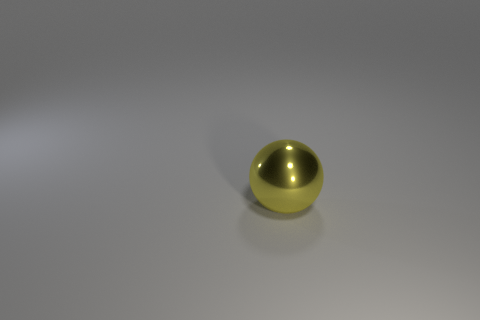
\includegraphics[width=0.43\linewidth]{figures/CLEVR_single.png}
        \label{fig:clevr-single}
    }
    \subfigure['CLEVR color', \emph{small brown cylinder}]{
        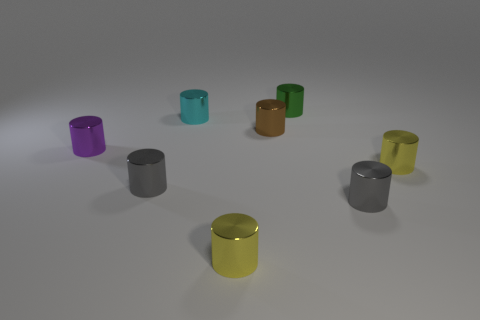
\includegraphics[width=0.43\linewidth]{figures/CLEVR_color.png}
        \label{fig:clevr-color}
    }
    \subfigure['Dale-2', \emph{small green cylinder}]{
        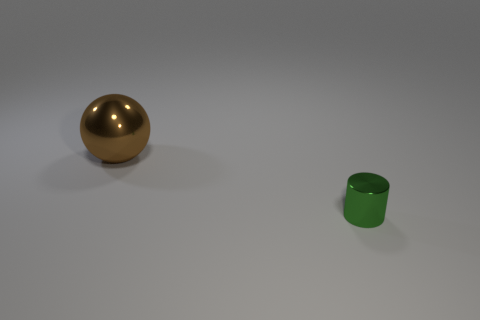
\includegraphics[width=0.43\linewidth]{figures/CLEVR_dale-2.png}
        \label{fig:clevr-dale-2}
    }
    \subfigure['Dale-5', \emph{large purple cylinder}]{
        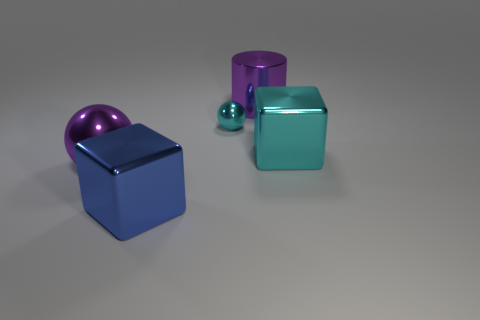
\includegraphics[width=0.43\linewidth]{figures/CLEVR_dale-5.png}
        \label{fig:clevr-dale-5}
    }
    \caption{Example images of each dataset, with the target object specified}
    \label{fig:clevr-examples}
\end{figure}

\subsubsection*{CLEVR single}
The simplest new dataset is called 'CLEVR single'.
This is a very simple dataset and has the purpose to simplify the problem the model needs to learn as much as possible.
Each scene in the dataset contains only one single object, the target object.
There are neither objects in the target nor in the distractor group.
All attributes are assigned randomly to the target object.
The differences across the whole dataset are the locations and rotations of the objects.
With this dataset, neural models can focus on only the features, as well as the locations of this single object.
There are no objects that distract the model from extracting features from the target object.
This helps to understand if the models are actually able to assign features or learn locations of these features in an image.
Figure \ref{fig:clevr-single} shows an example with the only object being the \emph{large yellow sphere}.

\subsubsection*{CLEVR color}
The second dataset that is created is called 'CLEVR color'.
The purpose of this dataset is to create scenes, where the target object is completely unique and as easily identifiable as possible.
For this reason, there exist only two groups in the scene, the target object and distractors.
The distractor group can contain in between 6 and 9 objects.
To make the discrimination as simple as possible the target object and the objects in the target group share exactly two attributes.
Furthermore, to simplify the relation between target object and distractors over the whole dataset, it is also controlled which attributes are shared.
The distractors have always the same size and shape as the target object, but the color is different.
The reason for choosing the color as the only discriminating attribute is that it is assumed that the color is easier to learn for neural models as opposed to for instance abstract shapes.

As seen in Figure \ref{fig:clevr-color}, the \emph{small brown cylinder} is unique.
By this, it is possible to refer to the target object using the attributes with four different combinations: the \emph{brown} object, the \emph{brown cylinder}, the \emph{small brown} object and the \emph{small brown cylinder}.
All attributes, apart from the color are not discriminating the target object from the distractors.
Notice as well that this restriction doesn't apply to the distractors, where multiple objects with the same color are allowed.

\subsubsection*{CLEVR Dale datasets}
The above described dataset is very restrictive on the disambiguating relations between the target object and the rest of the objects.
The number and the type of shared attributes are controlled exactly.
More realistically would be if objects can share a variable number of attributes.
In real situations, there is no restriction at all how objects or things relate to each other.
Natural language emerged that can refer to distinct attributes of these objects to discriminate them from each other.
This emergence of referring attributes and their combination is studied deeper in this work.

For this, I created a dataset that allows almost any relation between a target object and the distractors.
The relations are only restricted by the incremental algorithm for the Generation of Referring Expressions (GRE) described in \citet{Dale1995}.
This algorithm ensures that every scene contains a unique object in respect to its and the distractors' attributes.
Using the algorithm, one can refer to an object using its attributes to discriminate it from all other objects as efficiently as possible.
In other words, the object is described unambiguously using the lowest number of words.
For the dataset that means that zero, one or two attributes can be shared between the target object and distractor objects.
This ensures the uniqueness of the target object.
On the other side, it is not controlled which attributes are shared.
These are assigned randomly.
There is again no control over the relations between distractors, which means that distractors can appear multiple times.

Two datasets following these rules are created.
The Dale-2 dataset contains one target object and one distractor (see Figure \ref{fig:clevr-dale-2}), while the Dale-5 dataset contains one target object and exactly four distractors.
Consider Figure \ref{fig:clevr-dale-5}, with the target object being the \emph{large purple cylinder}. The large purple sphere shares the size and color, the two cubes only share the size, and the small turquoise sphere doesn't share any attribute.

These two datasets allow a more realistic look in how models can acquire knowledge about attributes of objects.
More specifically it helps to understand how models learn to discriminate objects from each other, since the model may only need to learn discriminative features of objects and not all features of the whole object.

\cmtDK{probabilities of shared attributes for both Dale-2 and Dale-5}

\subsection{Generating and understanding referring expressions}
\label{sec:preexperiments}
This chapter serves two purposes.
First, the generated dataset from the precious section is validated.
For this, models are trained to both generate referring expressions of the target object and understand existing referring expressions.
A success of these experiments indicates that the target objects in the datasets are possible to refer to and the datasets can be used in more complex setups in language games.

Secondly, the experiments in this chapter provide the basis for the setup of the agents in the language games.
Language games are very complex setups for machine learning models.
The models need to solve multiple tasks at the same time in order to solve the overall problem.
For instance, in a simple setup of a game two agents are involved.
The first agent, the sender, is shown a scene with objects and needs to communicate one target object to the other agent, the receiver.
The receiver is shown the same scene and needs to identify the target object with respect to the message of the sender.
In this case, the sender first needs to learn to encode the scene, all objects and their attributes, as well as the information about the target object into its own game specific space.
In a next step it needs to learn how to translate this encoding into a message that is sent to the receiver.
The receiver then needs to learn to decode this message, after which it needs to learn how to combine the decoded message with its own encoding of the scene and objects.
And finally it needs to learn how to identify the target object with this information.
There are many points of possible failure to train the agents.

For this reason, I decided to divide the main problem and let the models learn simpler subtasks and increase the complexity step by step.\footnote{\href{https://github.com/DominikKuenkele/MLT\_Master-Thesis}{https://github.com/DominikKuenkele/MLT\_Master-Thesis}}
This will give a very detailed overview where the models struggle to learn and in which ways they can be improved.
Mainly, the tasks are I separated into language games with two agents and classical machine learning tasks without any communication, namely only one 'agent' that solves the task alone.
With this division, I can analyze the learning of the encodings of the scenes separately from the learning of producing and decoding messages.

The final objective of this thesis is to find out, how agents can communicate about relations of objects based on their attributes, namely how to generate and understand referring expressions.
Because of that, the first experiments focus on extracting information from images and combining them with structured knowledge about the objects.
Here, I structured the experiments into three levels.
In the first level, the models are trained to learn the position of objects in the image and attend to specific regions of the image, by understanding a referring expression of the target object.
In the second level, the models are trained to differentiate objects in the scene from each other, again by understanding referring expressions.
In the last level, the models are trained to generate referring expressions, more specifically the models learn to caption and describe objects in the image.
These combined experiments should lay the basis for how to build up the agents in the language games.

\subsubsection{Coordinate predictor}
\label{sec:coordinate_predictor}
\subsubsection*{Setup}

This level should help to analyze, how the final task of the language game should look like, in especially what the receiver is tasked to predict.
As described before, the sender should communicate an object in the image and the receiver needs to identify it.
The challenge lies in how the receiver refers to the identified object.
There are multiple possibilities, how it can be done.
One of them could be to describe the target object with human language, using the attributes.
The main goal however is to let the language of the agents emerge as natural as possible.
Including human knowledge into the task would bias also the emerged language towards attributes and words, used in natural language.
For this reason, the final task of the receiver will be to 'point' to the target object.
The models are therefore tasked to predict the center coordinates of the target object.
With this approach, the models receive few human knowledge, but are still able to rely on all information present in the image to discriminate the objects.

To achieve this goal, multiple setups of models are tested.
In the simplest setup, the model receives only the image \cmtDK{preprocess image} as an input and produces two numbers as an output, the predicted x- and y-coordinate of the target object.
Here the image is first passed through one of the \emph{feature extractors}.
Next, the extracted feature vector is flattened and passed through two linear layers with a \emph{ReLU} non-linearity in between.
These reduce the dimensions first to 1024 and finally to 2.

To determine the loss, the euclidean distance between the resulting predicted point on the image and the ground truth point are calculated.
This distance is learned to be minimized.
By doing that, the model learns to focus and attend on a specific part in the image, in a perfect model the center of the target objects.

With this simple setup, the model is theoretically able to focus on an object in the image.
The problem arises as soon as multiple objects are present in the image.
There is no information available for the model to understand which one of these objects is the actual target object, except for the final calculation of the loss.
Since there is not necessarily a pattern for which object in the image is the correct target object over the whole dataset, the models will likely fail to generalize.
Therefore, the models need to receive more information.
Here, I try out four different ways to encode and refer to the target object.

\begin{figure}[h]
    \centering
    \subfigure[Model including one-hot encoded attributes and locations]{
        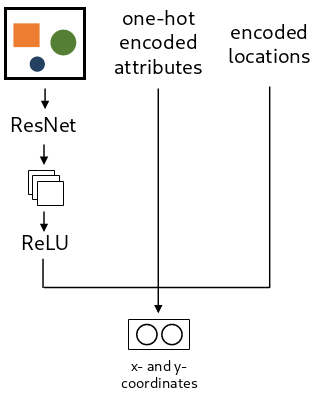
\includegraphics[width=0.35\linewidth]{figures/arch_coordinate_predictor.png}
        \label{fig:coordinate_predictor_architecture}
    }
    \subfigure[Model including GRE description]{
        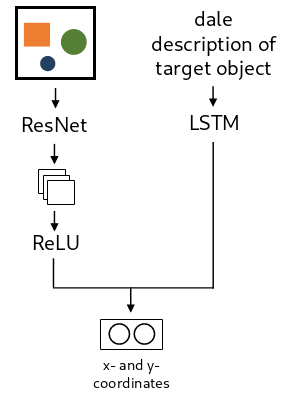
\includegraphics[width=0.315\linewidth]{figures/arch_coordinate_predictor_dale.png}
        \label{fig:coordinate_predictor_dale_architecture}
    }
    \caption{Simplified architecture of the coordinate predictors}
\end{figure}

In the first method, I encode the attributes of the target object as \textbf{one-hot encodings}.
There is a three-dimensional vector encoding the \emph{shape}, an eight-dimensional vector encoding the color and a two-dimensional vector encoding the two different sizes.
The values of each dimension of these vectors can either be zero or one, depending on the attributes of the target object.
These three encodings of the attributes are then concatenated.
The image is again passed through a feature extractor, before the flattened vector is reduced to 2048 dimensions with a linear layer.
The result is concatenated with the encoded attributes and passed to a final linear layer to predict the coordinates.

In an extension to this method, I also include the \textbf{center coordinates of all objects} in the image.
This should help the model to identify all possible options to chose from, when predicting the target object.
All the center coordinates are simply extracted and shuffled.
Since there are varying numbers of objects in the image, this vector of variable length is padded to the maximum number of objects in the dataset.
The padded locations consist of two zeros for both coordinates.
For this model, I also made use of a more complex way to encode the image.
Here, I based the approach on code that implements baselines for the CLEVR dataset \citep{Johnson2017}.
The image is first passed through the feature extractor.
Afterwards, a 2-dimensional convolutional layer, reduces the channels from 2048 to 512 channels with a kernel size of 1.
After applying the \emph{ReLU} function, the resulting matrix is max pooled over two dimensions with both a kernel size and a stride of 2.
The resulting matrix is flattened and concatenated with both the attribute encodings and the shuffled coordinates of all objects.
This is then passed again through a final linear layer to predict x- and y-coordinates.

The third method encodes the attributes of the target object with human language using the \textbf{incremental algorithm for the Generation of Referring Expressions (GRE)} described in \citet{Dale1995}.
This opposes the idea described before, to share as few human knowledge as possible with the model.
Still, this approach can help to understand and analyze if the model was able to extract information about the objects and more specifically their attributes from the image.
If the model is able to match parts of the image with human words it would show that the model learned this attribute.
If the model in a next step can learn this for the whole dataset, this would mean that it could generalize over these attributes and assign them to certain regions in an image.
This insight would help for succeeding models that make use of these learnings without human language.

Using the algorithm, one can describe an object using its attributes to discriminate it from other objects as efficiently as possible.
In other words, the object is described unambiguously using the lowest number of words.
The algorithm assumes that there is an order of importance for attributes, such as shape, color and size.
This order defines, which attributes can be left out, while still identifying the object uniquely.
This research relies on the following order from most important to least important: shape, color, size
Given for example the scene from \ref{fig:clevr-dale-5} with the target object being the \emph{big purple cylinder}.
Using all three attributes, this description identifies the object perfectly and uniquely.
Following the algorithm, we could make the description shorter by removing the least important attribute \emph{size} without loosing unambiguity, describing it as the \emph{purple cylinder}.
This can be taken even one step further by removing also the \emph{color}.
Describing it as the \emph{cylinder} still doesn't describe any distractor, since the target object is the only cylinder in the scene.

For the experiments, each image is captioned with a description of the target object using the described algorithm.
To include it in the model, the captions need to be padded to an equal length.
In this case they are padded to a length of 3, which is the maximum number of attributes that can be used.
For this, as standard practice in captioning tasks, the captions are padded at the end with a specified padding token.

The model is made up of three parts:
The first part extracts features from the image.
Here, the setup is similar to the previous model.
The image is passed through a feature extractor, before it is passed through two 2d convolutional layers, both reducing the channels to 128 with a kernel size of 1.
A \emph{ReLU} function is applied, after both convolutional layers.
As before, the resulting vector is pooled, using max pooling with both a kernel size and stride of 2.
In the second part, the caption is encoded, using an LSTM.
Here, the learned embeddings of each token are parsed by the LSTM and its final hidden state is then used as a summary of the complete caption.
The third part is again the predictor of the coordinates of the target object.
Both the processed image and the final hidden state of the LSTM are flattened and concatenated.
The resulting vector is passed through three linear layers reducing to 1024, 1024 and 2 dimensions respectively.
Between each linear layer, the \emph{ReLU} function is applied.
This architecture is also inspired by the baselines described in \citet{Johnson2017}.

The forth method, to encode the target object utilizes \textbf{masking} of the image.
For this, the image is separated into a fixed size squared area containing the target object and the rest of the image.
The side of the square is always two fifth of the image width, in this case 192 pixels.
This size always includes the whole object if it is large or small, while not being cut off if the target object is too close to the border of the image.
The square is filled in white, while the rest of the image is filled in black.
This approach has the advantage of providing as few as possible human bias to the model.
While even the one-hot encodings contain human knowledge by explicitly encoding human chosen attributes, masking the image will only point the model towards the target object without giving more information.
It therefore can only rely on its own extracted visual features when looking at masked images.
The model is presented with both the original image and the masked image.
Both are passed through a feature extractor and afterwards passed through a linear layer, reducing the dimensions to 2048.
The resulting vectors are concatenated and passed through another linear layer that predicts the coordinates.

The test dataset is again evaluated on the euclidean distance of the predicted coordinates to the ground truth coordinates.
This distance needs to be minimized.
The mean of all calculated distances is calculated across the whole epoch, which results in a mean distance score per epoch.
Since this score only takes the average of all predictions into account it doesn't show how every prediction fared individually.
If for instance the prediction of one object is getting more precise with growing number of epochs, but the precision of another object gets worse, the mean distance will stay the same.
It doesn't reflect this change.
For that reason, I also introduced an accuracy score.
For that I defined a fixed size circle with a radius of 20 pixels around the center of each object.
If the model's prediction lies in this circle, it will be counted as a correct prediction, if it lies outside, it is a false prediction.
These scores are averaged for the epoch and result in an accuracy score, where 100\% means that all predictions were very close to the center coordinates and 0\% means that no predictions were close to the center coordinates.
This of course doesn't give a perfect representation since the size of the objects varies, but it will still show, how precise each individual prediction is.
A high accuracy may indicate that the model could identify this specific object better.

The coordinate predictors are trained on the 'CLEVR single' as well as on both 'Dale' datasets.
The 'CLEVR single' dataset should test the model if it can actually learn locations of an object.
Since the model relies on the extracted features of either VGG or ResNet, locational information about the image could have gone lost.
Training on this dataset should make sure that the model can converge towards the correct pixels, utilizing these features.
In a next step, the 'Dale' datasets provide the actual problem of discriminating objects from each other and afterwards pointing to the correct one.
Here, the models should make use of the additional given referring expressions about the scene, as one-hot encodings of the attributes, descriptions using the GRE-algorithm or the encoded locations.
'Dale-2' and 'Dale-5' provide two different difficulties for the model, where it needs to discriminate a target object from one or four distractors.
Latter task is assumed to be significantly harder.

\subsubsection*{Results}

\begin{figure}[h]
    \centering
    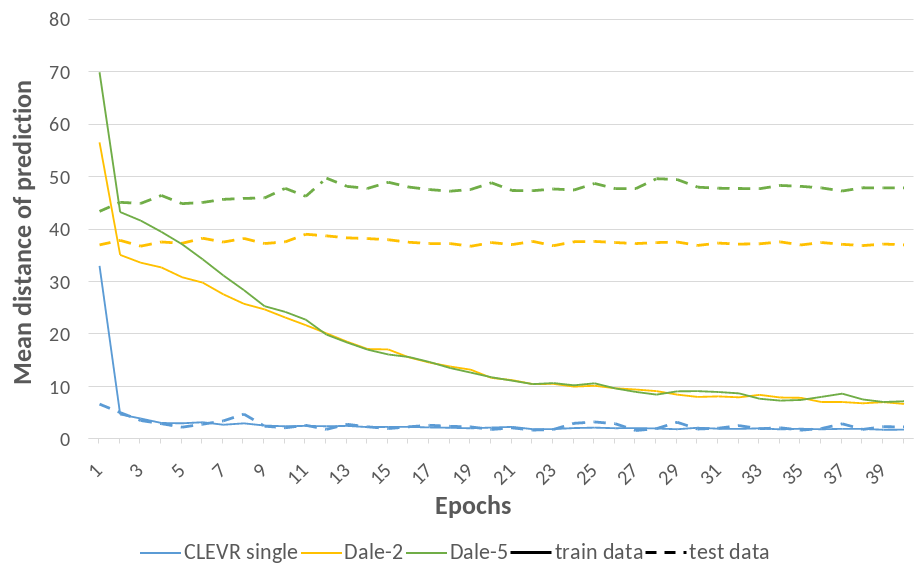
\includegraphics[width=0.8\linewidth]{figures/coordinate-predictor_loss.png}
    \caption{Mean distance between predicted coordinates and ground truth in pixels on different datasets}
    \label{fig:coordinate-predictor_loss}
\end{figure}

Figure \ref{fig:coordinate-predictor_loss} shows the results of the coordinate predictor that doesn't include any information about the target object.
The used feature extractor for these results is \emph{Resnet-3}, but the results don't differ meaningfully from results with other feature extractors.
As can be seen, the success between the different datasets are significant.
The more objects are present in an image, the worse the model performs.
The model converges for the CLEVR single dataset after around 20 epochs to a mean distance of around 2 pixels.
This prediction even though not perfectly on the center point is always on the object.
Opposed to that, using the Dale-2 dataset with two objects, the mean distance lies between 37 and 38 pixels already after the first epoch and doesn't drop with increasing number of epochs.
With five objects in the Dale-5 dataset, the model only predicts a mean distance of around 45 pixels in the beginning, which worsens with a rising number of epochs to 48 pixels.

An interesting observation is the difference of the mean distances between training and testing data.
The training distance is constantly approaching zero, while the testing loss is staying constant or even getting higher.
This points to the fact that the model is not generalizing the task by learning abstract patterns that can be applied to unseen data, but is instead memorizing the training data.
That is especially visible for the Dale-5 dataset, where learning the patterns of the training data looses even the ability to interpret some patterns in the testing data.
Applying a higher dropout didn't have an impact on the results.

This behavior is indeed not very surprising.
First, results with the 'CLEVR single' dataset show that the model is able to derive geometrical information from abstract feature, extracted by a feature extractor.
Geometrical information therefore doesn't get lost during this abstraction, but the model is able to point to a specific object, as long as only one object is part of the image.
Secondly, more than one objects present in an image confuses the model, and it is not able to consistently point to one of them.
This can have multiple reasons, for instance that the models lacks the ability to separate objects in the extracted features.
But even in case, the model is able to do that and could determine the location of each object in the scene given the feature, it would not be able to tell, which of these is the actual target object.
The guess is then more or less random.
This especially applies to the Dale-2 dataset, where an identification of the target object just based on one distractor is impossible; both of the present objects are unique.
For the Dale-5 dataset, the model could in theory learn that the target object is always the one object which is unique in respect to its and the distractors' attributes.
This task on the other hand seems very difficult to learn.
In conclusion, the models are able to predict geometrical coordinates, but need more information about the target object to identify it.

When the target object \textbf{attributes are encoded as one-hot vectors} and added to the input, the results don't improve.
One factor that now has a much higher impact is the feature extractor that is used.
Table \ref{tab:feature-extractor-mean-distances} compares the mean distances the models predict for the different feature extractors.
The results are shown for the models trained on the Dale-2 and Dale-5 datasets for training and test data.
First, a big difference can be seen between the datasets.
The models only converge to a minimum mean distance of around 46 pixels to the correct coordinates for the Dale-5 dataset, looking at the test data.
In most cases, it stays above 50 pixels.
Using the Dale-2 dataset, the behavior is a little different.
All ResNet extractors with four residual blocks and an additional average pooling and optionally a classifier layers reach similar scores as the experiments before without any one-hot encodings.
Interestingly, without the classifier layer, the model doesn't converge at all and the mean distances jump up and down between the epochs.
This effect also applies when using less residual blocks.
Using the VGG, only VGG-cls2 achieve a similar performance, while the others predict coordinates between 43 and 46 pixels away.

\begin{table}[h]
    \centering
    \begin{tabular}{rcccc}
        \toprule
                            & \multicolumn{2}{c}{\textbf{Dale-2}} & \multicolumn{2}{c}{\textbf{Dale-5}}                                   \\\cmidrule(lr){2-3}\cmidrule(lr){4-5}
                            & train                               & test                                & train          & test           \\\midrule
        \textbf{VGG-0}      & 30,27                               & 46,20                               & \textbf{32,17} & 54,40          \\
        \textbf{VGG-avg}    & \textbf{29,99}                      & 45,08                               & 32,32          & 52,67          \\
        \textbf{VGG-cls1}   & 37,99                               & 43,28                               & 46,57          & 50,75          \\
        \textbf{VGG-cls2}   & 38,87                               & \textbf{39,02}                      & 47,48          & 49,91          \\
        \textbf{VGG-cls3}   & 39,99                               & 44,32                               & 47,26          & \textbf{46,77} \\\midrule
        \textbf{ResNet-3}   & 78,26                               & 65,23                               & 92,07          & 91,12          \\
        \textbf{ResNet-4}   & 44,14                               & 55,24                               & \textbf{36,48} & 58,28          \\
        \textbf{ResNet-avg} & \textbf{33,06}                      & \textbf{39,18}                      & 47,64          & 46,38          \\
        \textbf{ResNet-cls} & 37,57                               & 38,10                               & 44,72          & \textbf{45,92} \\
        \bottomrule
    \end{tabular}
    \caption{Mean test losses for different feature extractors with one-hot attribute encodings after 20 epochs}
    \label{tab:feature-extractor-mean-distances}
\end{table}

Secondly, the training loss now looks also different.
In almost no cases, the models converge to a lower mean distance than with the test data, meaning a higher precision in their predictions, as they did in the experiment before.
The only exception is ResNet-3 as a feature extractor.
In other words, the models are again not able to generalize, but in specific cases memorize the patterns in the train data.
This hints to the fact that only specific layers of the feature extractors contain information that is generally usable to identify and discriminate objects.
Especially the lower layers with fewer residual blocks in the case of ResNet and no classifier layers for the VGG seem to not encode knowledge that can be utilized for this task.
Higher layers, with more specific encoded information need to be used for this research.
The experiments in the following sections are set up using these higher layers.

Adding \textbf{information about the center coordinates} of all objects should have helped the models to get a list of possible predictions.
In theory, the model could learn to choose between these coordinates by relating them to the extracted features of the image.
This hypothesis doesn't hold.
All results for both datasets Dale-2 and Dale-5 are the exact same as without included information about the locations.
The problem therefore doesn't seem to lie in predicting coordinates in general, but predicting the coordinates of the target object.
The model is still not able to understand, which object is the target object.
For that reason, a better representation of the target object is necessary.

In a next step, information about the attributes is included using the \textbf{\emph{GRE-algorithm}} from \citet{Dale1995}.
Again, the mean distance of the predictions as well as the accuracy doesn't improve compared to the previous experiments.

\begin{figure}[h]
    \centering
    \subfigure['Dale-2', train split]{
        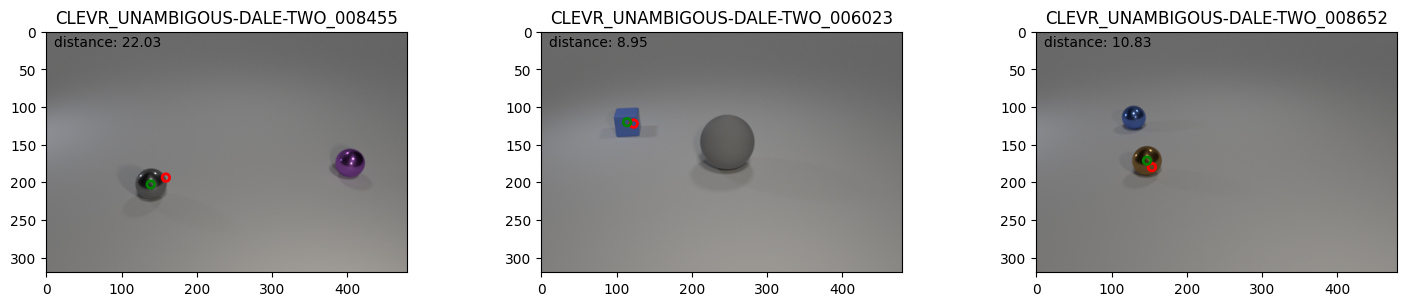
\includegraphics[width=.92\linewidth]{figures/visualization_dale-2_train.png}
        \label{fig:visualizations_dale-2_train}
    }
    \subfigure['Dale-2', test split]{
        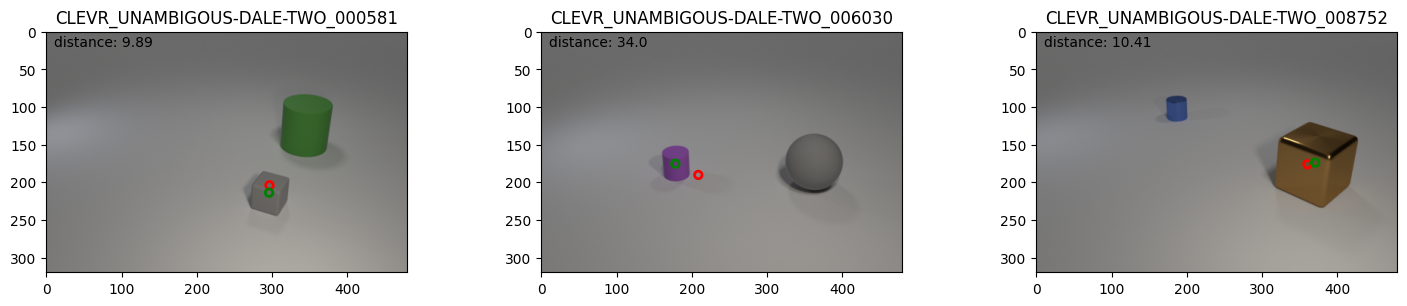
\includegraphics[width=.92\linewidth]{figures/visualization_dale-2_test.png}
        \label{fig:visualizations_dale-2_test}
    }
    \subfigure['Dale-5', train split]{
        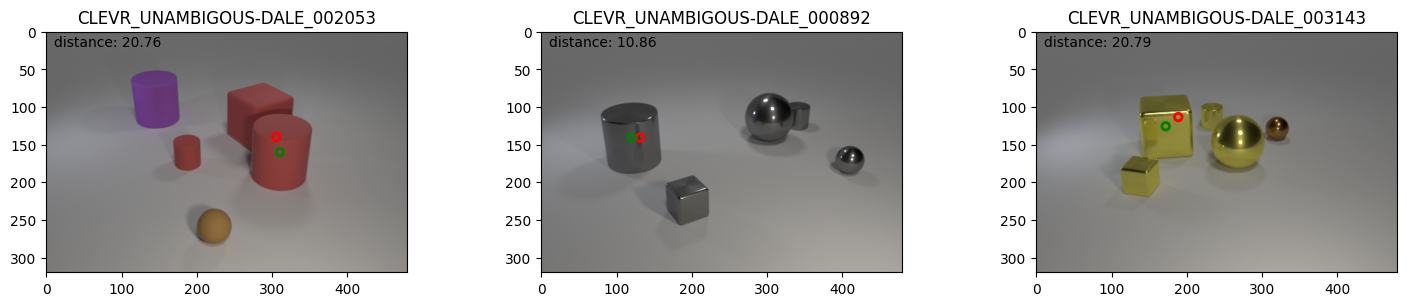
\includegraphics[width=.92\linewidth]{figures/visualization_dale-5_train.png}
        \label{fig:visualizations_dale-5_train}
    }
    \subfigure['Dale-5', test split]{
        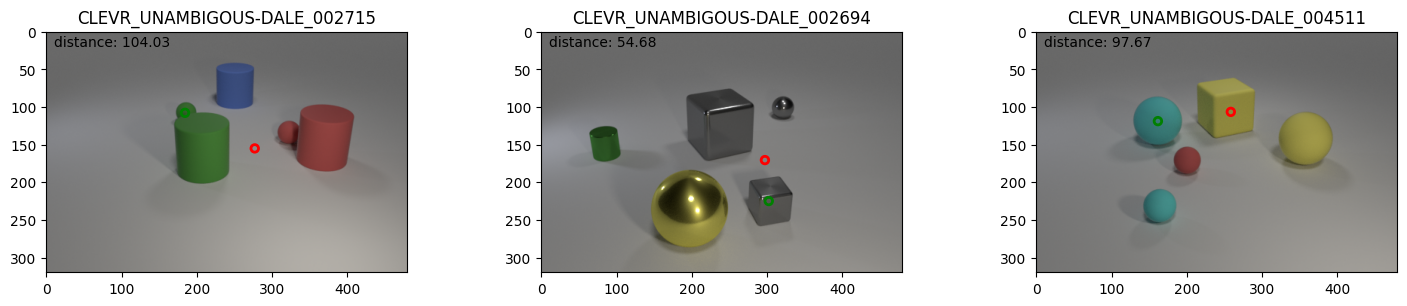
\includegraphics[width=.92\linewidth]{figures/visualization_dale-5_test.png}
        \label{fig:visualizations_dale-5_test}
    }
    \caption{Visualization of the models' predictions in the 'Dale' datasets}
    \label{fig:visualizations_dale}
\end{figure}

An interesting pattern appears when doing a qualitative analysis of the models' predictions.
Here, I visualized the predicted coordinates compared to the ground truth coordinates.
Figure \ref{fig:visualizations_dale-2_train} shows random examples of predictions for images in the train dataset of Dale-2.
The green circle shows the ground truth center coordinates of the target object, while the red circle shows the prediction of the model.
As can be seen, the predictions are very precise.
Figure \ref{fig:visualizations_dale-2_complete_train} combines the predictions and ground truths across all images in the train dataset.
Here, all predicted coordinates are placed as red circles into the image, while all ground truth coordinates are placed as green circles.
The resulting shape is a rhombus, which reflects that all objects are placed usually central into the scene.
As expected the green and red rhombus align mostly in the same area for the train split of the 'Dale-2' dataset.

The results look very different for the test split.
As can be seen in Figure \ref{fig:visualizations_dale-2_test}, the three randomly selected predictions don't align with the ground truth coordinates.
For all the images, the predictions don't lie on any object.
In the left image as well as in the central image, the predictions are closer to the target object than towards the distractor, but are still quite imprecise.
These findings align with the mean distance scores, described in the sections before.
However, it seems that the model's predictions are all towards the center of the image.
This can be seen clearer in Figure \ref{fig:visualizations_dale-2_complete_test}.
Again, the green circles form the shape of rhombus.
In contrast, the predictions in red almost all cluster in the center of the image.
They form roughly the shape of a smaller rhombus.
This behavior can be observed for all datasets and architectures of the model.
Figures \ref{fig:visualizations_dale-5_train}, \ref{fig:visualizations_dale-5_test}, \ref{fig:visualizations_dale-5_complete_train} and \ref{fig:visualizations_dale-5_complete_test} show the results for the 'Dale-5' dataset.
Here, the model more likely predicts the center coordinates of a distractor object as seen in the right image, which is also reflected in the lower score of the mean distance.
Also the combined visualization shows the same clustering of predictions in the center of the scene, but the pattern of the smaller rhombus is more visible.

\begin{figure}[h]
    \centering
    \subfigure['Dale-2', train split]{
        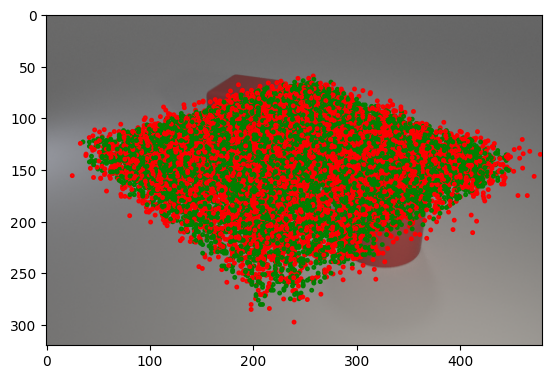
\includegraphics[width=0.42\linewidth]{figures/visualization_dale-2_train_complete.png}
        \label{fig:visualizations_dale-2_complete_train}
    }
    \subfigure['Dale-2', test split]{
        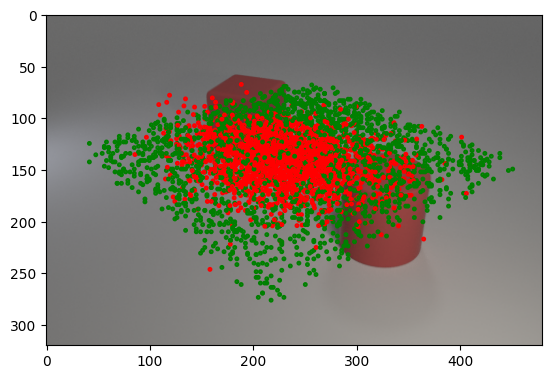
\includegraphics[width=0.42\linewidth]{figures/visualization_dale-2_test_complete.png}
        \label{fig:visualizations_dale-2_complete_test}
    }
    \subfigure['Dale-5', train split]{
        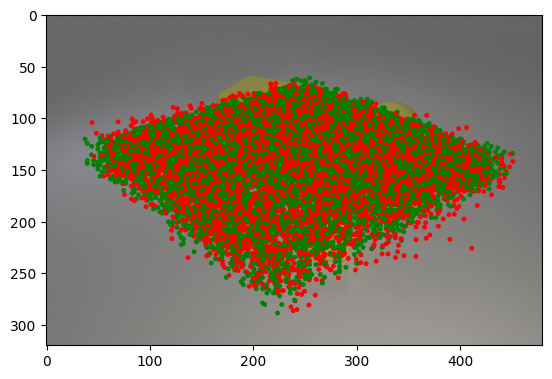
\includegraphics[width=0.42\linewidth]{figures/visualization_dale-5_train_complete.png}
        \label{fig:visualizations_dale-5_complete_train}
    }
    \subfigure['Dale-5', test split]{
        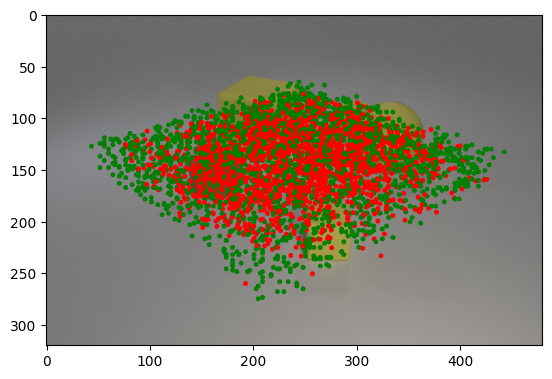
\includegraphics[width=0.42\linewidth]{figures/visualization_dale-5_test_complete.png}
        \label{fig:visualizations_dale-5_complete_test}
    }
    \caption{Visualization of the models' predictions in the Dale datasets}
    \label{fig:visualizations_dale_complete}
\end{figure}

These results allow two conclusions.
First, the models are biased to predict coordinates in the center of the image.
The reason for this is likely that the model can produce a relatively low loss, without relying on many extracted features of the objects.
Since all objects are always located in the center of the image and never in its corners, a prediction of any coordinate in the center is on average closer to the target object than any random prediction or predictions of coordinates at the borders of the image.
The model therefore learns only, where any object is likely located and can minimize the mean distance to a certain extent with this strategy.

Second, even though the models are biased towards the center of the image, the predictions are still often leaning towards the location where many objects lie.
This can be seen for the 'Dale-5' dataset, especially in left and central image in Figure \ref{fig:visualizations_dale-5_test}.
Again, by this strategy, the model can minimize the mean distance, since the probability is high that the target object lies in this cluster of objects.
Concluding, the model is able to extract, where objects are located in the image, but can't make use of the referring expressions, to decide which of these objects is the target object.

\subsubsection{Bounding box classifier}
\subsubsection*{Setup}
\cmtDK{better to call it discriminators?}

One problem that arises, when only predicting the coordinates is that the models may not be able to predict locations of objects from just visual features.
Feature extractors like VGG or ResNet are trained on extracting visual information.
In this process, absolute locations of these features in the images may get lost in the resulting vectors, since they are not necessarily important for classifying tasks.
To address this challenge, I restructured the task in this experiment.
Instead of predicting two coordinates of a target object, the model now needs to classify between all available objects, target object and distractors.
This will take all positional information out and just focus on the attributes and discriminating factors between the objects.
To do this, fixed-size bounding boxes are extracted around each of the object in the image.
As for the masking in the experiment before, the bounding boxes are a square of 192x192 pixels to capture the complete object.
The bounding boxes of all objects are padded to the maximum number of objects present in an image across the whole dataset with a matrix of zeros.
For the 'Dale-2', this corresponds to a maximum of two bounding boxes, 5 bounding boxes for the 'Dale-5' dataset and 10 for the 'CLEVR color' dataset
These bounding boxes are shuffled.
Furthermore, to point the model towards the target object, its attributes are encoded as on-hot vectors.

\begin{figure}[h]
    \centering
    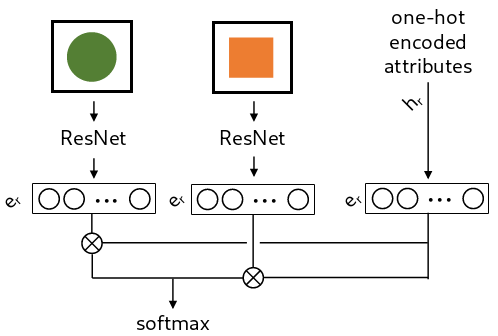
\includegraphics[width=.5\linewidth]{figures/arch_bounding_box_classifier.png}
    \caption{Simplified architecture of the bounding box classifier}
    \label{fig:bounding_box_classifier_architecture}
\end{figure}

The model passes each of the bounding boxes through a linear layer to transfer it into an embedding space of 10 dimensions.
The same is done with the one-hot vector of the target attributes.
In the next step, the dot product between each embedded image and the embedded attributes are calculated.
A high correlation between the attributes and the object should result in a high dot product, while a low correlation results in a lower dot product.
The model then points to an object, using the \emph{softmax} function over all concatenated dot products.
The loss is calculated using cross entropy.

Furthermore, the model is compared to a baseline that doesn't include any information about the target object.
Here, the model passes all flattened bounding box representations through a linear layer resulting in a vector with as many objects as are present in the image.
Again, the model uses a \emph{softmax} function to point to one of these objects.
Since no information about the target object is included, the guesses are expected to be random.

The bounding box classifier is trained on all datasets excluding the 'CLEVR single'.
The 'Dale' datasets are directly comparable to each other for the similar setup of their creation.
Especially interesting is the effect of the increasing the number of distractors and the growing number of attributes that are needed to discriminate the objects.

\subsubsection*{Results}
As expected, all baselines achieve a random accuracy for each of the datasets.
The accuracy lies at 50\% for the 'Dale-2' dataset, 22\% for the 'Dale-5' dataset and 12\% for the 'CLEVR color' dataset.
This changes however, when information about the target object is included.
Table \ref{tab:results_bounding_box_classifier} lists the accuracies of the models' predictions after 10 epochs.

\begin{table}[h]
    \centering
    \begin{tabular}{rcc}
        \toprule
                             & \textbf{Accuracy baseline} & \textbf{Accuracy} \\
        \textbf{Dale-2}      & 50\%                       & 99\%              \\
        \textbf{Dale-5}      & 22\%                       & 94\%              \\
        \textbf{CLEVR color} & 12\%                       & 93\%              \\
        \bottomrule
    \end{tabular}
    \caption{Results of the bounding box classifier after 10 epochs}
    \label{tab:results_bounding_box_classifier}
\end{table}

The model achieves almost perfect accuracy on the 'Dale-2' dataset with 99\%.
For both other datasets, the accuracy is slightly lower with 94\% and 93\% respectively, but still close to perfect, especially compared to the random baseline.
First, this shows that the model is able to extract attribute features from the image and manages to combine them with the given information about the target object.
This worsens slightly, when more objects are introduced.
More objects lead to more needed attributes to discriminate the objects from each other.
The model is still able to extract and utilize these additional attributes and combine them with the given attribute encoding of the target object.
The model can generate these high results, even with its relatively simple architecture.
In this architecture, the model doesn't compare the objects directly to each other, but each object is only associated with the attribute encodings.
A more complex architecture, in which the model is additionally tasked to discriminate the objects directly from each other might even improve the results.

\subsubsection{Caption generator}
\label{sec:caption_generator}
\subsubsection*{Setup}

As the bounding box classifier, the caption generator acts as a learning step towards understanding, how the model can learn the attributes of objects.
The same method using the GRE-algorithm from the section above is used to create the descriptions of the target object for each image.

There are some minor additions concerning the padding of the caption.
As before, the caption is padded to a number of three tokens, corresponding to the maximum of three attributes.
However, there are three different ways how the padding is applied.
First, the captions are, as usual in captioning tasks padded at the end with a specified padding token.
A problem could arise when the caption is not viewed as a natural language sentence, but as slots filled with tokens.
More specifically, following the GRE-algorithm, the last token in the caption is always the shape.
The second last token if existing describes the color, while the third last token if existing describes the size.
As soon as this sequence is padded at the end, these slots suddenly disappear.
A caption that only describes the shape, such as \emph{cube} will be padded to \emph{cube <pad> <pad>}, where the third last slot is filled up with the shape instead of the size.
Since in this task we are not focussing on producing natural language with a correct grammar, but focus instead of extracting attributes, having a slot structure could help the model to express the extracted attributes correctly.
For this reason, the second method of padding the caption is prepending the caption with padding tokens.
By this, the positions of the slots are preserved and if not specified just filled with a padding token.
The last variation concerns the order of producing each token.
When the captions are prepended, the model would need first produce two padding tokens, before it finally can produce a much more meaningful token for the shape.
This could be difficult to learn for a model, as the longer a sequence of tokens is, the more information about the beginning of the sequence gets lost.
Even though a sequence of just three tokens may not be long enough for this factor to be a problem, I experimented to reverse the caption.
Instead of producing for instance \emph{<pad> green sphere} as correct in English, the model would now need to produce \emph{sphere green <pad>}.
Notice that the padding token is again at the end of the generation, but the order of slots as well as the amount of information in the caption are still preserved.

The task for the model is to generate these descriptions, based on the complete scene as input.
Doing this, the task inherently involves learning human knowledge and natural language structure.
Nonetheless, this helps to understand more detailed if and how the model discriminates objects.
Does it rely on the same attributes humans are using, or does it find other important differences, or is it not able to solve the task at all?

\begin{figure}[h]
    \centering
    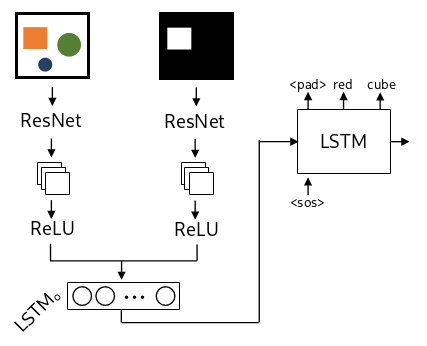
\includegraphics[width=.5\linewidth]{figures/arch_caption_generator.png}
    \caption{Simplified architecture of the masked caption generator}
    \label{fig:caption_generator_architecture}
\end{figure}

I compare two different models against each other.
The first model just takes the image as the input.
During training, also the ground truth caption is passed to the model.
The image is processed as in the section before.
First, it is passed through a feature extractor with two following 2d convolutional layers, reducing the channels to 128.
After each convolutional layer the \emph{ReLU} function is applied.
The result is pooled using max pooling and then reduced to 1024 dimension using a linear layer.
The such encoded image serves as the initial hidden state of an LSTM, which generates the caption.
During training teacher forcing is applied by using embeddings of the ground truth tokens as the input sequence for the LSTM.
The output of the LSTM is passed through a linear layer at each step to determine logits over the symbols of the vocabulary.
The loss is calculated using cross entropy.
During testing, the LSTM is always forced to generate three tokens, with an embedded start-of-sequence token as first input to the LSTM.
Each token in the sequence is determined, by selecting the highest logit in the output of each step in the LSTM.

Using this approach, the model doesn't have any information about the target object.
Therefore, I extend it in a second step with a masked image.
A masked version of the image is created ass in the section above and passed to the model.
This is shown in Figure \ref{fig:caption_generator_architecture}.
The model works exactly the same, except for the additional separate image encoder that encodes the masked image in the same way as the original image.
Both encodings are concatenated and then used as the initial hidden state for the LSTM.
This should point the model towards which object to describe and discriminate from the distractors.

To test the success of the model, three measures are calculated.
The first measure is the \textbf{accuracy} if the model predicted every word in the caption correctly.
This gives a hint, how the model fares in general and if it is able to predict any of the attributes.
However, a 'false' prediction doesn't give much insight into why the model predicted a wrong caption.

It could be the case that the model predicted the correct shape, but wrong color.
Even worse, the model could have predicted more attributes than necessary to uniquely identify the target object and didn't follow the rules of the GRE-algorithm.
For instance, consider the scene in Figure \ref{fig:clevr-dale-5}.
The correct caption is \emph{cylinder}.
If the model would predict \emph{purple cylinder}, the accuracy determines it as false as captioning \emph{large purple cylinder} as well \emph{small green cube}.
The first two descriptions identify the target object perfectly, but the model only didn't learn to exclude unnecessary attributes.
To mitigate this, I also include a \textbf{word-by-word accuracy}.
This measure calculates the accuracy not on sentence level, but on word level.
The first predicted caption of the model would yield a word-by-word accuracy of 66\% (including padding tokens), the second 33\%, while the third prediction would
yield 0\%.
This can give a better understanding of the errors the model makes.

With the \textbf{non-target accuracy}, I identify if the model described another object, which is not the target image.
This is basically an inverted accuracy score; the lower the score, the better the model fares.
For this I generated captions for all the non-target objects and distractors in the images using the GRE-algorithm.
If the generated description of the model describes an object that is not the target object, it gets assigned 100\%.
If not, independently of describing the target object, no object, or one of the objects insufficiently, it gets assigned 0\%.
Using this measure, I can get a quick overview if the model's problem lies in extracting and relating attributes or in understanding which of the presented objects is the target object.

The caption generator models are trained on both 'Dale' datasets.
Again, each of these datasets increases the complexity of the description.
While the referring expression for the 'Dale-2' datasets are generally shorter, expressions of the 'Dale-5' datasets need to be more specific and use more attributes.
Furthermore, the model needs to attend to many more locations in the image at the same time to find discriminating factors between those.

\subsubsection*{Results}
In the next paragraphs, the results of the caption generator will be discussed.
Table \ref{tab:results_caption-generator} shows the different scores of the models when trained on 'Dale-2' and 'Dale-5'.
ResNet-3 produced the best results, when it was used as a feature extractor.
The results are shown after 50 epochs, but the scores already start to converge after 20 epochs and changed only very little in the following epochs.

\begin{table}[h]
    \centering
    \begin{tabular}{rccc}
        \toprule
                               & \textbf{Accuracy} & \textbf{Word-by-word accuracy} & \textbf{Non-target accuracy} \\
        \textbf{Dale-2}        & 49\%              & 82\%                           & 48\%                         \\
        \textbf{Dale-2 masked} & 72\%              & 90\%                           & 25\%                         \\
        \textbf{Dale-5}        & 21\%              & 45\%                           & 40\%                         \\
        \textbf{Dale-5 masked} & 21\%              & 54\%                           & 45\%                         \\
        \bottomrule
    \end{tabular}
    \caption{Results of the caption generator, based on ResNet-3}
    \label{tab:results_caption-generator}
\end{table}

The sum of the \emph{accuracy} and the \emph{non-target-accuracy} adds to 97\%, when trained on the 'Dale-2' dataset.
This means that the models produce almost always correct descriptions of one of the objects in the image.
Moreover, these descriptions are also efficient in the sense that they follow the GRE-algorithm of \citet{Dale1995} and only use necessary discriminative attributes.
Features of both objects are therefore extracted perfectly and associated with the vocabulary.
As expected, the model has difficulties to decide, which of both objects is the target object, since no information is passed to the model.
With 48\% of the images describing the target object and 49\% of the images describing the distractor, the model uses a random guess.
This changes, when also the masked image is presented to the model.
Then, the accuracy for the target object rises with 72\% well above chance.
Still, the wrong descriptions describe almost every time the distractor object.
This indicates that the problem doesn't lie in extracting features of objects, but only in deciding which object in the image to describe.

When the model is trained on the 'Dale-5' dataset, the results are much worse.
Now, without masking only in 61\% of the images, the model describes any of the objects in the image.
With 21\% of these descriptions being a description of the target object, the model again uses a random guess.
Interestingly, passing the masked image to the model doesn't help it to identify the correct object.
The accuracy stays at the same value.
In contrast, the non-target accuracy is increased by 5\% points.
The model is more likely to identify a wrong object.
Furthermore, the word-by-word accuracy increases from 45\% to 54\%.
This increase is likely due to the fact that the description of the target object often shares some attributes with distractor objects.
For instance an image with a target object being a \emph{small red cube} was identified as a \emph{<pad> <pad> cube} when the model didn't receive the masked image.
When also the masked image is passed to the model, it generates the description \emph{small blue cube}.
This was the correct description of a distractor and because of the overlap of the attributes, the word-by-word accuracy increased from 33\% to 66\%.

The approach, how the padding is produced and in which order the attributes are concatenated didn't have an effect on the described metrics.
When the order was reversed and the padding appended, the model was converging slightly faster and reached the limit around two to three epochs earlier.
The final peak stayed exactly the same and the effects were therefore not studied deeper.

There are two main possible explanations for the big difference between the two datasets.
First, as already seen in the experiments before, the bigger number of distractors confuses the model more, where to focus on.
In the 'Dale-2' dataset, there are only two possibilities, while the four distractors in the 'Dale-5' dataset give the model a bigger choice.
The second explanation lies in the used GRE-algorithm.
When only two random objects are placed in a scene, the probability that only the shape is enough to discriminate the objects is at 66,6\%, namely the caption is only one word long.
For shape and color, the probability lies at 29,2\% and that all three attributes are necessary is 4,1\%.
Opposed to that the probabilities with four distractors are 19,8\%, 47\% and 33,2\% respectively.
With four distractors the algorithm is much more likely to produce longer captions.
These are harder to learn and generate for the model since it needs to take more extracted attributes into account to discriminate the target object from the distractors.

\subsection{Language games}
\label{sec:language-games}

The experiments that are executed using language games have a similar structure as the experiments in the previous chapters, since those provided the basis for the language games.

The language games in this research have an asymmetric setup.
One agent, the sender is shown some information and needs to generate a message.
This message is received by the second agent, the receiver.
The receiver needs to parse this message and combine it with the same information that the sender was presented with.
The receiver then makes a prediction, which is compared to the ground truth.
The game is set up prosocial, which means that both agents receive the same loss based on the receiver's prediction.
All weights of the agents are adapted in the same way.

The vocabulary that the sender can draw from to produce a message is made up of initially arbitrary symbols.
The meaning of these symbols is created as soon as the sender uses them in one of the message, and the receiver is able to use it to solve the task successfully.
Over time, specific meanings are reinforced and a language emerges.
The number of possible words, namely the size of the vocabulary can be varied.

First, I will discuss \emph{discrimination games}, because they have the simplest setup.
Furthermore, other language games that research this topic use a very similar setup.
In the next step, I will describe \emph{caption generators} that are set up as a language game.
Here, the sender describes the scene, while the receiver needs to generate a caption.
In the last step, I try to lose as much human bias as possible and the models are trained on just 'pointing' towards the target object, by again predicting its center coordinates.

The languages that emerge are analyzed in two ways.
An analysis of the frequency of used symbols and messages, as well as an examination for which images and objects they are used indicates the structure of the language and meanings of the symbols.
In a second step, the language is compared to several referring expressions in natural language.
By doing this, it can be seen if the models learned to use similar ways of referring to objects as humans do, or if they rely on different approaches.

\subsubsection{Discrimination games}
\subsubsection*{Setup}

In a discrimination game, the agents are presented with two or more images, one of these being the target image.
The sender needs to communicate this target image to the receiver by discriminating it from the other distractor images.
The receiver then needs to decide based on the message, which of the images is the target image.

The discrimination games in this research have a very similar setup as described in \citet{Lazaridou2017}.
The agents in this research resemble their \emph{agnostic sender} as well as their \emph{receiver}.
One central difference is the production of the message.
The main goal of their language game was the identification of the concept that and image was related to.
Therefore, the sender communicated only single-symbol messages to the receiver, which should describe the concept of the target image.
Opposed to that in this research, the agents are tasked to discriminate objects from each other based on their attributes.
It is therefore assumed that the sender will communicate these discriminative attributes.
For that reason, the sender is allowed to generate sequences as a message.

Both 'Dale' datasets are used to train the agents in this mode.
Similarly to the bounding box classifier, bounding boxes around each of the objects are extracted and fed to the game.
As in \citet{Lazaridou2017}, the sender receives the bounding box of the target object as the first image, while the rest of the bounding boxes are shuffled.
The sender is assumed to learn which of the input images is the target images by this approach.
The receiver receives the images in completely shuffled order.

\begin{figure}[h]
    \centering
    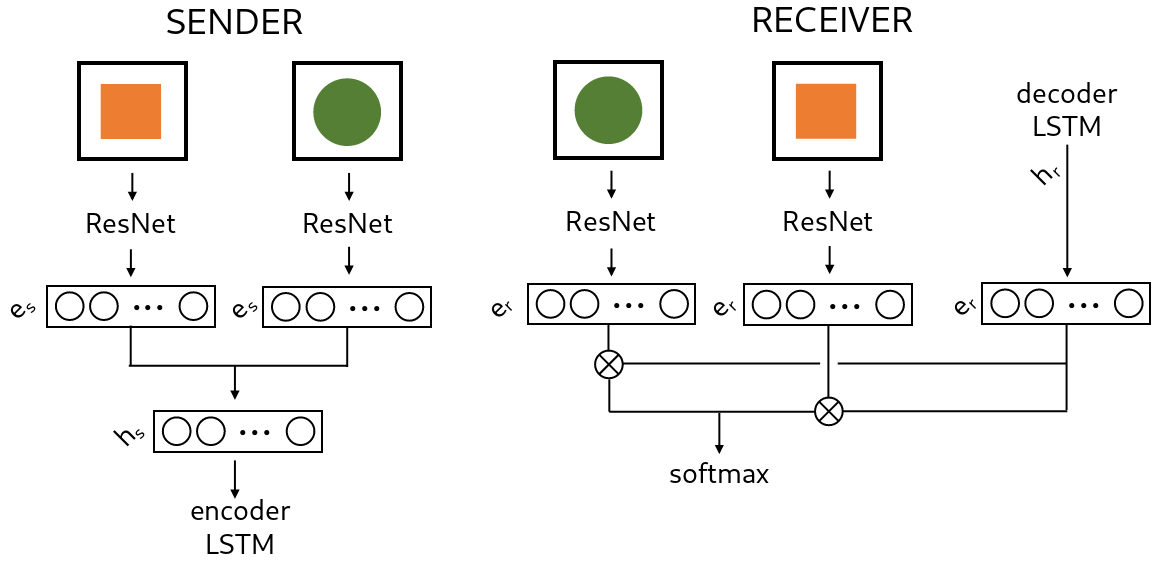
\includegraphics[width=.8\linewidth]{figures/arch_discriminator.png}
    \caption{Sender and receiver architectures in the discrimination game}
    \label{fig:discriminator_architecture}
\end{figure}

Figure \ref{fig:discriminator_architecture} shows, how the sender and the receiver of the discriminator are built up.
For the sender, the images are passed through a feature extractor and a following linear layer that reduces the dimensions to an embedding size $e_s$.
All embedded images are concatenated and passed through another linear layer to reduce the dimensions to the hidden size $h_s$.
This is then used as the initial state of the encoder LSTM in the sender wrapper.

The receiver also encodes all images using a feature extractor with a following linear layer, reducing it to $e_r$.
The sequence, received by the sender is the input for its decoder LSTM, where the hidden state with a dimension of $h_r$ is randomly initialized.
As mentioned above, the receiver combines this image representation with the hidden state of each symbol separately.
This is done by passing the hidden state through a linear layer to scale its dimensions to the same $e_r$.
This allows the calculation of the dot product between it and the image representation.
If the message describes an object well, the resulting dot product should be higher.
The receiver then `points' to one of the images by applying the \emph{softmax} function over the results of the dot products.
The loss is calculated using the NLL-loss.

During the experiments, five variables are adjusted to compare their effects:
(1) the image embedding size for the sender $e_s$, (2) the LSTM hidden size for the sender wrapper $h_s$, (3) the image/message embedding size for the receiver $e_r$, (4) the LSTM hidden size for the receiver wrapper $h_r$ and (5) the size of the vocabulary $|V|$.

\subsubsection*{Results}
Table \ref{tab:results_discriminator} shows the accuracy of the models calculated on the success of communication if the receiver can identify the target object.
A random guess corresponds to 50\% in the \emph{Dale-2} dataset and 20\% in the \emph{Dale-5} dataset.
Four different vocabulary sizes $|V|$ are tested.
A size of 13 symbols corresponds to the 13 attributes the objects can have and align with human language.
If the symbols were similarly used, messages would have lengths between one and three symbols.
Opposed to that a slightly smaller vocabulary with 10 symbols is used to create a smaller bottleneck with a higher pressure to condense the information.
Similarly, a bigger vocabulary consisting of 20 symbols tests how a bigger bottleneck changes the results.
Lastly, a big vocabulary of 100 symbols should give the model all options to encode the information, including one symbol per attribute or one symbol describing a combination of attributes.

The hidden sizes $h_s$ and $h_r$ as well as the embedding sizes $e_s$ and $e_r$ are chosen in alignment with the vocabulary size.
The hidden sizes are always smaller or equal to the vocabulary size since the information about each word needs to be compressed in a smaller dimension to learn meaning.
Hereby, hidden sizes of 10 and 100 are tested.
On the other hand, three different embedding sizes are tested: 10, 50 and 100.
The reason for this is to experiment, what is the optimal middle ground between compressing features of an image encoded in high dimension vectors and upscaling encoded messages in low dimension vectors.

\begin{table}[h]
    \centering
    \begin{tabular}{ccccc|cc|cc|cc}
        \toprule
              &         &         &         &         & \multicolumn{2}{c}{\textbf{Dale-2}} & \multicolumn{2}{c}{\textbf{Dale-5}} & \multicolumn{2}{c}{\textbf{CLEVR color}}                                                         \\\cmidrule(lr){6-7}\cmidrule(lr){8-9}\cmidrule(lr){10-11}
        $|V|$ & $h_{s}$ & $h_{r}$ & $e_{s}$ & $e_{r}$ & \textbf{Accuracy}                   & \textbf{length}                     & \textbf{Accuracy}                        & \textbf{length} & \textbf{Accuracy} & \textbf{length} \\\midrule
        {10}  & {10}    & {10}    & {10}    & {10}    & {96,4\%}                            & {0,99}                              & {24,7\%}                                 & {0}             & {17,3\%}          & {1}             \\
        {10}  & {50}    & {50}    & {50}    & {50}    & {50\%}                              & {1}                                 & {21,4\%}                                 & {1}             & {17,8\%}          & {0}             \\
        {13}  & {10}    & {10}    & {10}    & {10}    & {96,16\%}                           & {1}                                 & {24,8\%}                                 & {1}             & {17,1\%}          & {1}             \\
        {13}  & {10}    & {10}    & {50}    & {50}    & {49,6\%}                            & {1}                                 & {21,9\%}                                 & {1}             & {17,9\%}          & {0}             \\
        {20}  & {10}    & {10}    & {50}    & {50}    & {50,9\%}                            & {0}                                 & {23\%}                                   & {1}             & {15,9\%}          & {1}             \\
        {100} & {10}    & {10}    & {10}    & {10}    & {97,3\%}                            & {1}                                 & {24\%}                                   & {1}             & {18,1\%}          & {1}             \\
        {100} & {10}    & {10}    & {50}    & {50}    & {49,9\%}                            & {1}                                 & {24,4\%}                                 & {1}             & {15,8\%}          & {1}             \\
        {100} & {100}   & {100}   & {100}   & {100}   & {49\%}                              & {0}                                 & {25,3\%}                                 & {1}             & {15,6\%}          & {0}             \\
        \bottomrule
    \end{tabular}
    \caption{Results of the discriminators: $|V|$ are different vocabulary sizes, $h$ hidden sizes and $e$ embedding sizes.}
    \label{tab:results_discriminator}
\end{table}

For the \emph{Dale-2}, a clear correlation between the hidden sizes, embedding sizes and the size of the vocabulary can be identified.
A hidden/embedding size as high as the vocabulary size is beneficial for identifying the correct object.
The receiver identifies almost every sample correctly when all sizes are 10.
When the hidden and embedding sizes are increased, the guesses by the receiver are random with 50\% accuracy.
Interestingly, a vocabulary size of 10 is enough to communicate a meaningful message when the model is trained on the \emph{Dale-2} dataset.

The results change, when using the \emph{Dale-5} dataset with four distractors.
With four distractors and with low hidden, embedding and vocabulary sizes, the agents barely pass the random baseline with 23\%.
Only increasing the vocabulary size to 100 raises the accuracy by almost 20\% points to 43\%.
This is still considerably lower than the 95\% of the \emph{Dale-2} dataset.
The same applies to the 'CLEVR color' dataset, where all models achieve a very low accuracy of around 15 to 17\%, corresponding to random guesses.

\cmtDK{calculation of loss?}
\cmtDK{length}

Two conclusions can be drawn.
First, the hidden as well as the embedding sizes need to be close to the vocabulary size.
This even applies for very low vocabulary sizes, which means that the image encodings need to be compressed to the same low dimensions.
The reason for this is very likely that neural models have difficulties to upscale from lower dimensions (e.g. from low $h_r$ to high $e_r$) as opposed to learn how to extract the important information from a vector with many dimensions.

The second conclusion that can be drawn looks at the differences between the two datasets.
Unsurprisingly, the agents have a much higher difficulty to discriminate a target object from four instead of one distractor.
Since we discriminate objects based on properties that are also distinguished in human cognition (color, size, shape), we expect that the vocabulary onto which the agents converge reflects these categories and is therefore close to human vocabulary.
There are 48 possible combinations of attributes.
Still, for Dale-2, a vocabulary size of only 10 is enough for an almost perfect accuracy with two objects.
This hints to the fact that the agents don't describe the complete target object, but only rely on discriminative attributes between the objects.
The need for a more detailed description of discriminative attributes is higher when more distractors are involved.
Therefore, the models need to learn more combinations of symbols in order to attest to this higher level of detail and especially how to relate them to features in the images.

\cmtDK{similarity to bounding box classifier}

\subsubsection*{Analysis of the emerged languages}
In the above experiments, only three configurations lead to success, where a language emerged that the agents used to exchange information: languages with vocabulary sizes of $|V| = 10$, $|V| = 13$ and $|V| = 100$.
They will be referred to as $Lang_{10}$, $Lang_{13}$ and $Lang_{100}$ respectively.
In this section, these three emerged languages is analyzed in more detail.
This is done in two parts.
The first part is a qualitative analysis, to understand, which symbols are used to transfer which information.
In the second part, the emerged languages are compared to English.
More specifically, it is tested if the messages of the sender align with English referring expressions of the target object.

\begin{figure}[h]
    \centering
    \subfigure[$Lang_{10}$]{
        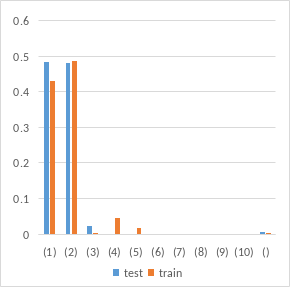
\includegraphics[width=0.31\linewidth]{figures/relative_frequencies_v10.png}
        \label{fig:relative_frequencies_v10}
    }
    \subfigure[$Lang_{13}$]{
        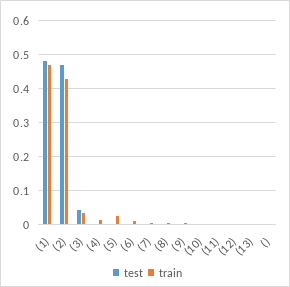
\includegraphics[width=0.31\linewidth]{figures/relative_frequencies_v13.png}
        \label{fig:relative_frequencies_v13}
    }
    \subfigure[$Lang_{100}$, (13 most frequent messages)]{
        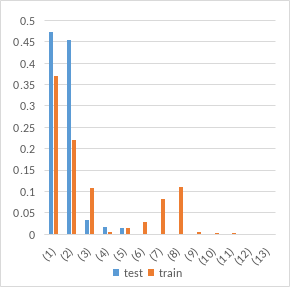
\includegraphics[width=0.31\linewidth]{figures/relative_frequencies_v100.png}
        \label{fig:relative_frequencies_v100}
    }
    \caption{Relative frequencies of messages (ordered by frequency in test dataset)}
    \label{fig:relative_frequencies_vocabularies}
\end{figure}

When looking at the emerged vocabulary \textbf{qualitatively}, a few properties can be seen.
Figure \ref{fig:relative_frequencies_vocabularies} shows an overview of the frequencies of messages in all three emerged languages for the training and the test split.
Since the tokens themselves are arbitrary, they are ordered by the relative frequency in the messages for the test set and indices for the tokens are added from index 1 for the most frequent token and index $|V|$ for the least frequent token.
By this the languages are easier comparable across different runs and vocabulary sizes.
Figure \ref{fig:relative_frequencies_v100} shows only the 13 most frequent message to provide a better overview.
The lesser frequent messages are never used for the test data and each only used one or two times in the train data.

The first property is that when a message is transferred, it consists of only one symbol.
In some rare cases, also an empty message is communicated.
The models therefore don't learn any compositionality by combining symbols to create new meaning, but rather encode everything in separate symbols.
Secondly, in all three languages, only very few symbols occur with a high frequency, while most of the symbols are used very rarely.
More specifically, two symbols are used in 95\% of the images with $Lang_{10}$ and $Lang_{13}$, while three symbols are used with $Lang_{100}$.
Thirdly, the agents make use of fewer symbols, when presented with unseen test images compared to when communicating about images in the training split.
This is especially visible for $Lang_{100}$.
Symbols that are used for 16,5\% of the training sample are not used at all in test split.
Furthermore, the frequencies in the test split is much more focused on the two most frequent symbols, while it is more distributed around 5 symbols in the train split.

These findings indicate that referring expressions do emerge in each of the newly emerged languages since the agents are able to communicate the correct object.
However, the agents converge towards very few different referring expressions that are made up differently than in English and likely don't rely on the high level attributes \emph{shape}, \emph{color} and \emph{size}.
The similar frequencies across all three languages suggest that a greater vocabulary size $|V|$ doesn't necessarily lead to different referring expressions, but the languages still converge towards two main expressions.

\begin{figure}[h]
    \centering
    \subfigure[$Lang_{10}$]{
        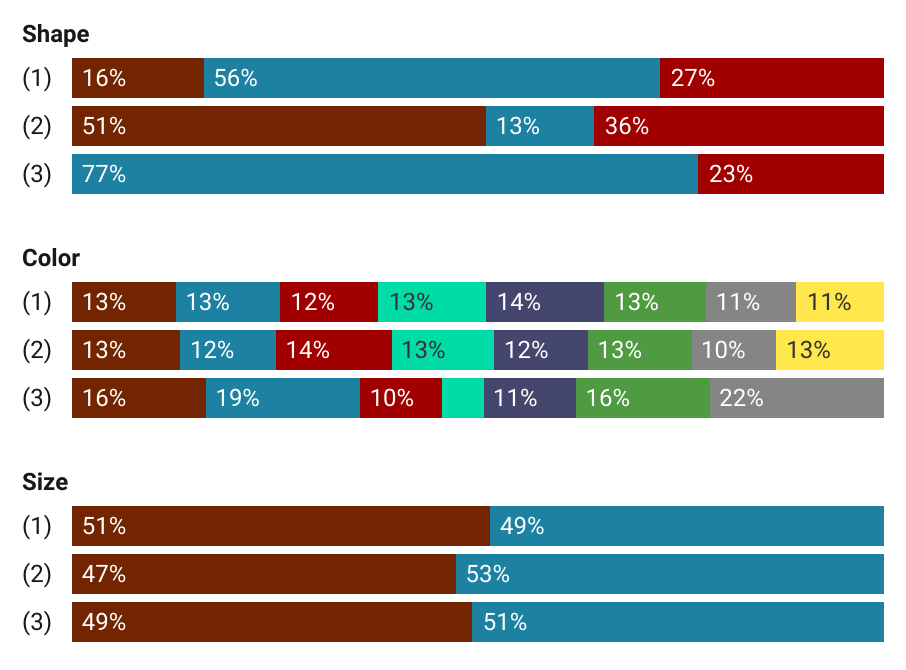
\includegraphics[width=0.31\linewidth]{figures/language_analysis_v10.png}
        \label{fig:language_analysis_v10}
    }
    \subfigure[$Lang_{13}$]{
        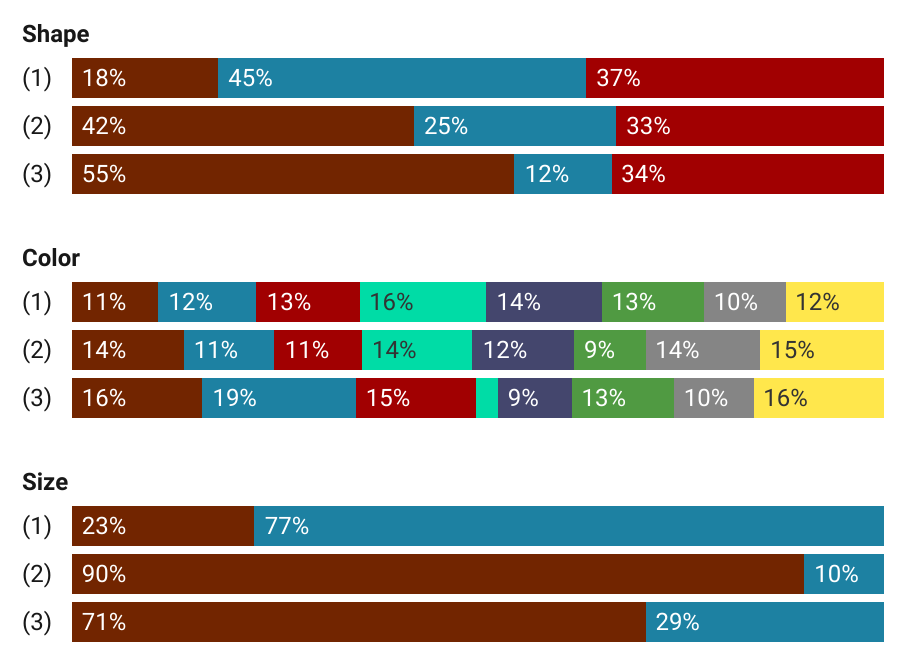
\includegraphics[width=0.31\linewidth]{figures/language_analysis_v13.png}
        \label{fig:language_analysis_v13}
    }
    \subfigure[$Lang_{100}$]{
        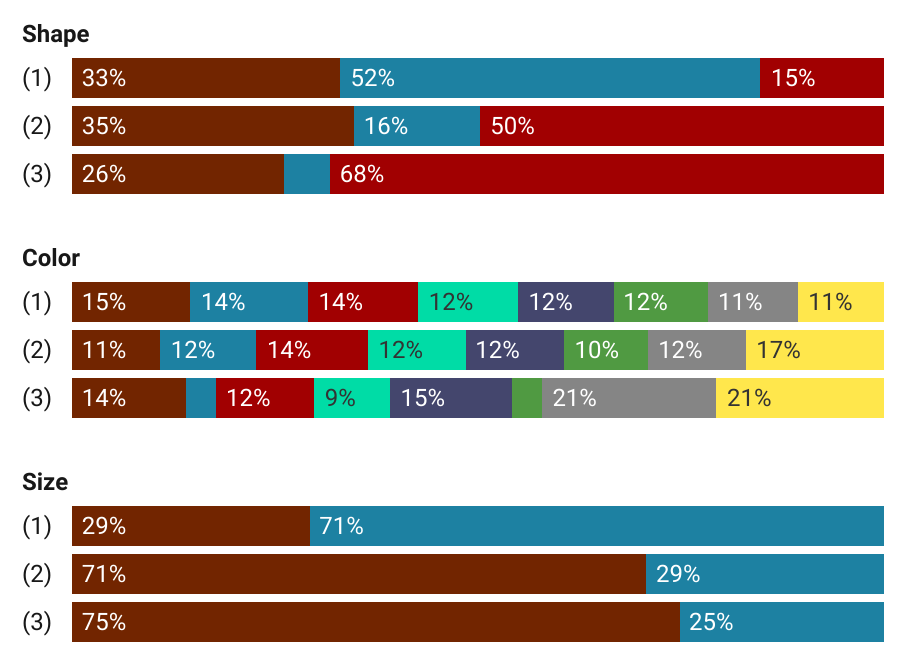
\includegraphics[width=0.31\linewidth]{figures/language_analysis_v100.png}
        \label{fig:language_analysis_v100}
    }
    \caption{Relative share of the described target object's attributes for the top three messages}

    \textbf{Shape:} brown: sphere, blue: cube, red: cylinder \\
    \textbf{Size:} brown: small, blue: large
    \label{fig:language_analysis_vocabularies}
\end{figure}

Figure \ref{fig:language_analysis_vocabularies} shows the attributes of the target object that are described by each message.
Hereby, the relative share each value of all three attributes are displayed.
For instance the first bar in Figure \ref{fig:language_analysis_v10} shows that 16\% of the target objects that are described with symbol (1) in the language $Lang_{10}$ are spheres.
In the figures, only the three most frequently used messages are included, which make up over 95\% of all messages.

The first thing that can be seen is that different symbols convey different values of attributes.
In the language $Lang_{10}$, symbol (1) is mostly used for target objects that are cubes, while symbol (2) is mostly used for spheres.
There is not much difference for target objects that are cylinders.
The distribution for colors is almost constant across symbols (1) and (2).
Symbol (3) is more frequently used for blue, green and gray objects, while being less used for red, cyan and yellow objects.
This different distribution may also be caused by the much lower absolute usage of symbol (3).
The different sizes are encoded by all symbols in the same way.

Looking at $Lang_{13}$ the symbol usage differs.
The frequencies for the shape look similar, but (the much less used) symbol (3) encodes most of the time spheres instead of cubes.
Again, the colors look similar with small deviations for brown, green and yellow objects.
Most striking however, is the difference for the size.
Symbol (1) is used in 77\% of the cases for large objects, while symbol (2) and (3) are used in 90\% and 71\% of the messages for small objects.

Language $Lang_{100}$ uses symbols its symbols to discriminate cubes and cylinders, while the frequencies for sphere remain constant across all symbols.
The usage for the color is similar to $Lang_{13}$.
Looking at the size, as for $Lang_{13}$, symbol (1) is mostly used to encode small objects, while symbols (2) and (3) are mostly used to encode large objects.

An interesting observation is that symbols are not used for the same attributes across the languages.
In some languages, an attribute is not captured at all by the symbols, while another language heavily relies on it.
The same applies to the values of attributes, especially to the shapes.
Only two of the shapes are distinguished by the usage of symbols, while the third is not captured.
Which shape are encoded, differs from language to language.

Furthermore, these numbers confirm even more that the agents don't rely solely on the human defined attributes.
For instance $Lang_{10}$ only encodes the shape in its symbols.
This would not be enough to distinguish the target object from the distractor consistently.
Following, the agents also encode some additional underlying attributes and patterns to the three above defined attributes.

To compare the emerged language to English in a \textbf{quantitative} way, a probing approach is used.
Probing can be used to analyze and interpret the hidden representations in neural networks.
Hereby, a second neural model is trained to predict selected linguistic properties on the basis of the hidden representations.
If this model is successfully able to predict the linguistic properties, the hidden representations are connected to them.
If second model can't be trained, it indicates that there is no correlation between the hidden representation and the linguistic property.
In the case of the emerged language, a neural model is trained to translate the messages of the sender into English referring expressions, based on the GRE algorithm by \citet{Dale1995}.
Hereby, the model consists of an encoder LSTM, one linear layer and a decoder LSTM.
The encoder LSTM encodes the messages of the emerged language.
The final hidden state is used as the meaning of the complete sentence and passed through the linear layer, which should learn an abstract representation of the message.
The resulting vector is used as the initial state of the decoder LSTM.
The decoder LSTM is then trained to produce the English referring expression.
While decoding, teacher forcing is applied.
The success of the model is validated calculating cross entropy between the models predictions and the target English referring expression.
Since generalization doesn't play a role for probing, no dropout is applied and the model is trained and validated on the complete dataset; no test or validation split is used.

In the sections above, the attributes are ordered by importance in the way, it is usually used in English: shape > color > size.
Since the agents do not necessarily need to follow this, all possible orders of importance for the attributes are compared to each other.

The translation model with this setup can learn two characteristics.
First, it can learn to find correlations between the emerged language and the English referring expressions.
Secondly, it can learn patterns in the English referring expressions that are independent of the emerged language.
For instance, it can learn that the referring expressions are likely to be two symbols long, or that 'cube' is the most common shape.
This second characteristic can lead to a low loss of the model, even though there are no connections to the emerged language.
In this test, only the first characteristic is interesting and would show the correlation between the emerged language and English referring expressions.
For that reason, two reference key numbers are calculated for each of the attribute importance order.
The first reference uses a non-informative input for the encoder LSTM, more specifically it always receives a vector of zeros and therefore can't learn any meaningful representation in the linear layer; the input for the decoder LSTM is the same for every sample.
By this, the model is trained to learn the patterns in the English referring expressions.
The resulting loss is the highest possible loss the model can achieve, independent of the input.
Resulting, if the emergent language is connected to English, the loss will be lower than this baseline.
If not, the loss will be as high as this baseline.
On the other side, I calculated the lowest loss possible, by using the English referring expressions as both input and target.
This verifies that the model is able to learn an abstract representation from the input and the resulting loss should be close to zero (since input is perfectly correlated to the target).
These two references are used, to normalize the results of the actual emergent languages $L_{em}$, using the formula $L_{norm} = \frac{L_{em}-L_{English}}{L_{baseline} - L_{English}}$.
A loss close as $L_{baseline}$ will lead to 100\%, while a loss as $L_{English}$ will lead to 0\%.
By doing this, all configurations can be compared directly to each other.

\begin{table}[h]
    \centering
    \begin{tabular}{c|cc|cc|cc|cc}
        \toprule
        \textbf{Order}          & $L_{baseline}$ & $L_{English}$ & \multicolumn{2}{c}{$|V| = 10$} & \multicolumn{2}{c}{$|V| = 13$} & \multicolumn{2}{c}{$|V| = 100$}                                                      \\\cmidrule(lr){4-5}\cmidrule(lr){6-7}\cmidrule(lr){8-9}
                                &                &               & $L_{em}$                       & $L_{norm}$                     & $L_{em}$                        & $L_{norm}$         & $L_{em}$ & $L_{norm}$         \\\midrule
        {shape > color > size}  & {0,659}        & {0,0001}      & {0,569}                        & \textbf{86,19\%}               & {0,622}                         & {94,24\%}          & {0,597}  & {90,4\%}           \\
        {shape > size > color}  & {0,589}        & {0,0002}      & {0,489}                        & \textbf{83,09\%}               & {0,531}                         & {90,21\%}          & {0,47}   & {\textbf{79,78\%}} \\
        {color > shape > size}  & {0,849}        & {0,0}         & {0,802}                        & 94,49\%                        & {0,801}                         & {94,36\%}          & {0,791}  & {93,15\%}          \\
        {color  > size > shape} & {0,836}        & {0,0}         & {0,819}                        & 98,01\%                        & {0,772}                         & {92,35\%}          & {0,786}  & {94\%}             \\
        {size > shape > color}  & {0,532}        & {0,0052}      & {0,492}                        & 92,26\%                        & {0,437}                         & {\textbf{81,95\%}} & {0,457}  & {\textbf{85,61\%}} \\
        {size > color > shape}  & {0,599}        & {0,0001}      & {0,573}                        & 95,71\%                        & {0,495}                         & {\textbf{82,67\%}} & {0,538}  & {\textbf{89,87\%}} \\
        \bottomrule
    \end{tabular}
    \caption{Cross entropy losses while probing with emerged languages successful on 'Dale-2'}
    \label{tab:probing_discrimnator_language}
\end{table}

Table \ref{tab:probing_discrimnator_language} shows the results for all different languages.
First, it can be seen for all emerged languages, the model is able to find correlations between natural language referring expressions and the messages by the sender.
Still, all losses stay high and closer to the loss of the baseline, namely where the model only learns the patterns in the English referring expressions.
This fact concludes that all emerged languages don't rely on the GRE algorithm by \citet{Dale1995}.
Nonetheless, it may be possible that a different algorithm is used to create referring expressions in the artificial language.

Secondly, it can be seen that the correlation between the emerged language and the natural language referring expressions differ for each of the languages.
The vocabulary consisting of 10 symbols is the closest related to the orders \emph{shape > size > color} and \emph{shape > color > size}, the vocabulary based on 13 symbols on the other hand to the orders \emph{size > shape > color} and \emph{size > color > shape}.
With 100 symbols, the vocabulary resembles mostly \emph{shape > size > color} and \emph{size > shape > color}.
Striking here is that even though the related orders are different, the most important attributes are either the \emph{size} or \emph{shape} across all three emerged languages.
The attribute \emph{color} seems to be less important.
This is reinforced by the fact that the losses are closer to the baseline, when the \emph{color} is the most or second most important attribute in the order.


\subsubsection{Caption generator games}
\subsubsection*{Setup}

In a next step, it is tested if the agents can learn to extract features of the objects together.
For this, the receiver is tasked to describe the target object in natural language, while the sender needs to communicate, which object is the target.
Again, the setup is asymmetrical: the sender receives the image and information, which of the objects in the image is the target object in form of a masked image.
The receiver only sees the image without additional information.
\cmtDK{human bias vs emergent language}

This setup is based on the single neural model described above.
The target caption for each image is created using the GRE-algorithm of \citet{Dale1995}.
Since the results of the experiments show that the position of the padding doesn't have an effect on the final converging scores, the padding tokens are only prepended to the caption.

\begin{figure}[h]
    \centering
    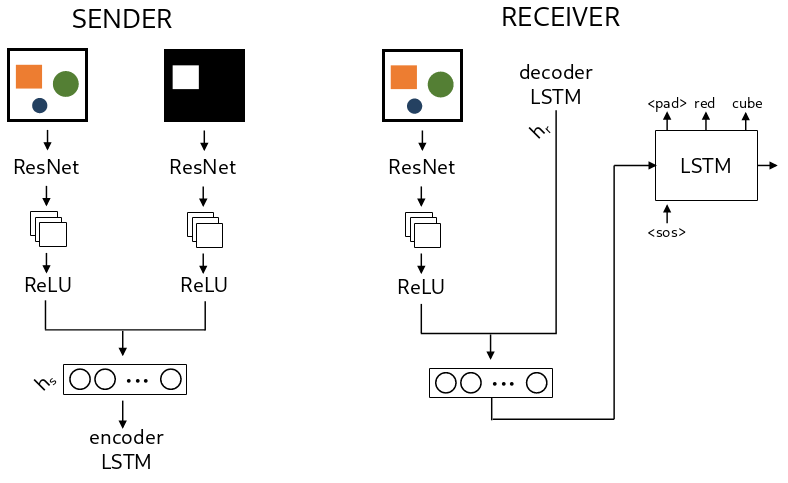
\includegraphics[width=.7\linewidth]{figures/arch_caption_generator_game.png}
    \caption{Simplified architecture of the caption generator game}
    \label{fig:caption_generator_game_architecture}
\end{figure}

The sender is built up of two image encoders, one encodes the original target image and one encodes the masked image.
The image encoders are set up as described in \citet{Johnson2017}.
A feature extractor extracts basic features of the images.
Two following convolutional layers with a \emph{ReLU} function are trained to condense the most important information from the resulting matrices.
A max pooling layer and a linear layer reduce the dimensions to 1024 dimensions.
This size was found to have the best results during the experiments.
The two resulting encoded images are flattened and concatenated.
A final linear layer reduces this long vector to the hidden size of the message LSTM $h_s$, which is used as the initial hidden state of this LSTM.

The receiver uses the same architecture to encode the original image as the sender.
The resulting flattened vector is concatenated with the decoded message of hidden size $h_r$.
This is then passed through a linear layer, again reducing it to 1024 dimensions and is then used as the initial state of the captioning LSTM.
During training, the ground truth caption is used as the input to the LSTM without teacher forcing.
When presented with test data, the LSTM always produces three tokens, by using its own predicted words as the input for the next step.
The loss is calculated with cross entropy.

Since the agents are trained to describe the target object discriminatively based on the described GRE-algorithm, they are trained on the 'Dale-2' and 'Dale-5' dataset.
The 'Dale-5' should be again much harder to learn, since there are more objects that the agents need to discriminate the target object from.

During the experiments, the following variables are adjusted, and the results are compared:
(1) the vocabulary size $|V|$,
(2) the LSTM hidden size of the sender wrapper $h_s$ and
(3) the LSTM hidden size of the receiver wrapper $h_r$.
The same metrics as in the pre-experiments are used to evaluate the results.

\subsubsection*{Results}
\begin{table}[h]
    \centering
    \begin{tabular}{ccc|ccc|ccc}
        \toprule
              &         &         & \multicolumn{3}{c}{\textbf{Dale-2}} & \multicolumn{3}{c}{\textbf{Dale-5}}                                                                             \\\cmidrule(lr){4-6}\cmidrule(lr){7-9}
        $|V|$ & $h_{s}$ & $h_{r}$ & \textbf{Acc.}                       & \textbf{word-by-word}               & \textbf{length} & \textbf{Acc.} & \textbf{word-by-word} & \textbf{length} \\\midrule
        {10}  & {10}    & {10}    & {22,9\%}                            & {62,8\%}                            & {1}             & {7,1\%}       & {40\%}                & {1}             \\
        {13}  & {10}    & {10}    & {22,8\%}                            & {62,9\%}                            & {0}             & {7,3\%}       & {38,7\%}              & {1}             \\
        {20}  & {10}    & {10}    & {24,6\%}                            & {64\%}                              & {1}             & {6,7\%}       & {38,7\%}              & {1}             \\
        {100} & {10}    & {10}    & {24,4\%}                            & {62\%}                              & {1}             & {7,8\%}       & {40\%}                & {1}             \\
        {100} & {100}   & {100}   & {21\%}                              & {62\%}                              & {1}             & {6,5\%}       & {37,8\%}              & {1}             \\
        \bottomrule
    \end{tabular}
    \caption{Results of the caption generator: $|V|$ are different vocabulary sizes and $h$ hidden sizes.}
    \label{tab:results_caption_generator_game}
\end{table}

The results of the caption generator game are summarized in Table \ref{tab:results_caption_generator_game}.
In general, it can be seen that the agents have much bigger problems, to solve the task together than a single neural network.
The highest accuracy for descriptions, the agents manage to predict correctly is at 24,6\% for images of the 'Dale-2' dataset.
Compared to the (masked) accuracy of the single model with 72\%, the agents predict 47,4\% points less correct descriptions.
A similar worse performance can be seen for the 'Dale-5' dataset.
Here, the agents only manage to produce for 7,8\% of the images correct descriptions, 13,2\% points less than the single neural model.
The same effect can be seen for the word-by-word accuracy, which is much lower than the metric for the single neural model for both datasets.

When looking, how the different variables affect the performance, it can be seen that a bigger vocabulary size tends to help the agents.
This is only visible for the 'Dale-2' dataset.
With constant hidden sizes of 10, the agents score around 22,9\% with only 10 and 13 available symbols.
When this is increased to 20 and respectively 100 symbols, the agents can increase their accuracy to around 24,5\%.
However, the increase is relatively small.
Interestingly, this effect only occurs, when the hidden sizes are small with only 10 dimensions.
As soon as they are increased to 100 dimensions with a vocabulary size of 100 symbols, the accuracy drops to 21\%.

Looking at the 'Dale-5' dataset, the increase is still there, when the vocabulary is increased to 100 symbols.
Nonetheless, the difference is with 0,5\% points even smaller and the reason may be due to other influences, such as the random initialization of the weights of the agents.
This is confirmed, when looking at emerged languages.
In all the setups, the same message is communicated for all samples, independently of the input image.
This is also reflected in the length of the messages.
For the setup with a vocabulary size of $|V| = 13$, no message is transferred, and the accuracy stays the same as in the other setups.

These results show that the agents are not at all able to encode meaning about the images and target objects in their messages.
This is especially interesting, compared to single model caption generator in section \ref{sec:caption_generator}.
In these experiments, the model was able to converge towards correct captions and therefore able to extract the necessary information.
This shows that a main challenge for the agents lies in grounding symbols in these extracted features.

\subsubsection{Coordinate predictor games}
\subsubsection*{Setup}
In the final experiments, it is tried to eliminate as much human knowledge as possible.
For that reason, the agents are tasked to only predict the location of the target object.
This task is approached in two steps.
In the first step the sender is still shown human knowledge in form of a description of the target object, since the previous experiments showed that the models were able to relate them to their own extracted features.
The receiver doesn't come in contact with any human knowledge, not as input nor as output.
This approach acts as a sanity check if the agents are able to converge together on the correct target object coordinates.
In the second step, the caption is also removed from the sender.
Instead, a masked image points the sender towards the target object.
In this setup, no human knowledge is explicitly present, that can bias the emerged language to form similarly to human language, except for the implicit information in the image itself.
With this, it can be analyzed, how the language between the agents emerges and which features or patterns are represented with symbols.

The agents are both set up in the same way as the single neural model, predicting the target object's coordinates.
The sender encodes the original image the same as in the previous paragraph.
In the first setup, the description of the target object is encoded, using an LSTM.
For this, an embedding with $emb_{descr}$ dimensions is learned to represent each word.
These embeddings are the input for the LSTM.
The final hidden state of $LSTM_{descr}$ dimensions is used as the representation of the whole description.
The vocabulary that is used for the descriptions is based on 14 symbols, including the padding token.
For the LSTM to learn a representation of each token as well as of the complete description, both $emb_{descr}$ and $LSTM_{descr}$ need to be smaller than the size of this vocabulary.
Choosing a size of 10 for both variables proved to give good results in the experiments.
In a next step, the image encoding and the final hidden state of the description are concatenated and passed through a linear layer to reduce the dimension to the hidden size $h_s$.
The resulting vector is passed to the sender wrapper LSTM, to generate the message.

\begin{figure}[h]
    \centering
    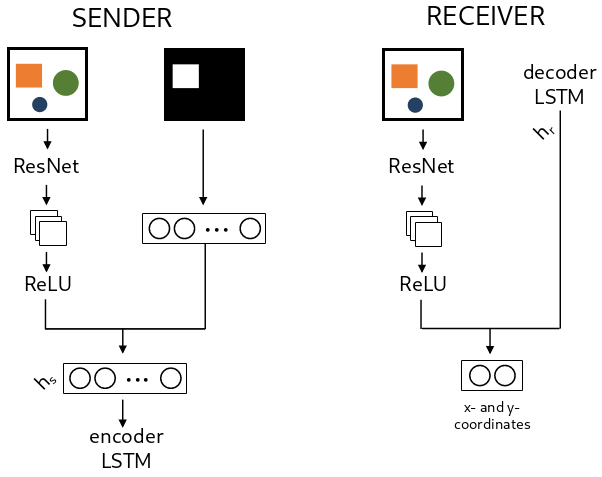
\includegraphics[width=.7\linewidth]{figures/arch_coordinate_predictor_game.png}
    \caption{Simplified architecture of the masked coordinate predictor game}
    \label{fig:coordinate_predictor_game_architecture}
\end{figure}

For the second approach, the masked image is passed only through a feature extractor.
Both the resulting encoding of the masked image and the encoding of the original image are each passed through separate linear layer to adjust their dimensions to the same embedding size $e_s$.
These embeddings are subsequently concatenated and reduced to the hidden size $h_s$ with a final linear layer.

The receiver contains of two parts.
First, the original image is encoded with an image encode of the same setup.
This encoded image is flattened and concatenated with the final hidden state of the wrapper LSTM encoding the message received by the receiver.
The resulting vector is the passed through the second part of the receiver, the predictor.
This predictor contains of three linear layers, reducing the dimensions to 1024, 1024 and 2 respectively.
A \emph{ReLU} function is applied in between.
This setup is trained to combine the important information from both the image and the message of the sender.
The euclidean distance between the resulting prediction of the center point and the true center of the target object is calculated and the weights of both agents are adapted accordingly.

As in the pre-experiments, the agents are trained first the 'CLEVR single' dataset to understand if they are capable of predicting locations in an image together.
In a next step, the 'Dale-2' and 'Dale-5' datasets are used to test if the agents are able to first communicate a target object and second describe the target object discriminatively with a small vocabulary.

During the experiments, the effects of the following variables are compared:
(1) the vocabulary size $|V|$,
(2) the LSTM hidden size of the sender wrapper $h_s$,
(3) the LSTM hidden size of the receiver wrapper $h_r$ and
(4) the embedding size of the sender $e_s$.
As before, the metrics to evaluate the results are the same as in the pre-experiments.

\subsubsection*{Results}
In the final setup, the agents are tasked with communicating objects with fewer infused human knowledge.
Table \ref{tab:results_dale_predictor_game} shows the results for the setup, in which the sender is pointed towards the target object with a human description based on the GRE algorithm.
Hereby, the 'CLEVR single' dataset acts as a baseline, to test if the agents are able to predict coordinates of objects at all.
In every configuration of the variables, the agents achieve a very high performance.
The worst average distance across the test dataset is 10 pixels, which still points onto an object.
Also the accuracy, which evaluates how many guesses of the receiver were pointing onto an object reflects this fact.
All configuration achieve an accuracy higher than 96,7\%.
This aligns also with the results from the single neural models, where the average distance was similarly low.
In general, this shows that the agents are able to predict coordinates together.
However, the question arises if the message by the sender has actually an effect on the receivers' decision, or if the receiver learns to point towards the target coordinates on his own and the message is ignored.
Having a look at the transferred messages, it in fact shows that the receiver learns to point towards the target object on its own.
As in the experiment before, all communicated messages contain the same symbol independent of the input image.

\begin{table}[h]
    \centering
    \begin{tabular}{ccc|ccc|ccc|ccc}
        \toprule
              &         &         & \multicolumn{3}{c}{\textbf{CLEVR single}} & \multicolumn{3}{c}{\textbf{Dale-2}} & \multicolumn{3}{c}{\textbf{Dale-5}}                                                                                                       \\\cmidrule(lr){4-6}\cmidrule(lr){7-9}\cmidrule(lr){10-12}
        $|V|$ & $h_{s}$ & $h_{r}$ & \textbf{Dist.}                            & \textbf{Acc.}                       & \textbf{length}                     & \textbf{Dist.} & \textbf{Acc.} & \textbf{length} & \textbf{Dist.} & \textbf{Acc.} & \textbf{length} \\\midrule
        {10}  & {10}    & {10}    & {10,1}                                    & {98,5\%}                            & {1}                                 & {36,5}         & {19,9\%}      & {1}             & {45,7}         & {14,4\%}      & {1}             \\
        {13}  & {10}    & {10}    & {6}                                       & {99\%}                              & {0}                                 & {38}           & {20,4\%}      & {1}             & {47,3}         & {10,8\%}      & {1}             \\
        {20}  & {10}    & {10}    & {9,7}                                     & {96,7\%}                            & {1}                                 & {37,3}         & {21,2\%}      & {1}             & {47,3}         & {11,3\%}      & {0}             \\
        {100} & {10}    & {10}    & {7,7}                                     & {98,4\%}                            & {1}                                 & {40,4}         & {21,7\%}      & {1}             & {45,4}         & {10,8\%}      & {1}             \\
        {100} & {100}   & {100}   & {7,5}                                     & {96,9\%}                            & {1}                                 & {40,1}         & {17,8\%}      & {1}             & {44,3}         & {11,8\%}      & {0}             \\
        \bottomrule
    \end{tabular}
    \caption{Results of the description coordinate predictor: $|V|$ are different vocabulary sizes and $h$ hidden sizes.}
    \label{tab:results_dale_predictor_game}
\end{table}

When the experiments are run on the 'Dale-2' dataset, the results are much worse.
For the \emph{description coordinate predictor}, the average distance ranges from 36,5 pixels to 40,4 pixels.
The configuration with a vocabulary size of only 10 symbols fares the best, while a vocabulary of 100 symbols produces the worst results.
Still, the accuracy shows that around 19,9\% to 21,7\% of the guesses are on the target object.
Here, the configurations with higher vocabulary sizes fare slightly better, but the differences are very small and likely due to other factors.

The results for 'Dale-5' dataset are even worse, but are comparable with the results with a single neural model.
Apparently, the agents are not able to communicate the target object, and the predictions by the receiver are general in the middle of the image, which results in an average distance of around 45 to 50 pixels.
The differences of the mean distances are not very significant in this range, to allow an analysis of the different configurations.

\begin{table}[h]
    \centering
    \begin{tabular}{cccc|ccc|ccc|ccc}
        \toprule
              &         &          &         & \multicolumn{3}{c}{\textbf{CLEVR single}} & \multicolumn{3}{c}{\textbf{Dale-2}} & \multicolumn{3}{c}{\textbf{Dale-5}}                                                                                                       \\\cmidrule(lr){5-7}\cmidrule(lr){8-10}\cmidrule(lr){11-13}
        $|V|$ & $h_{s}$ & $h_{r}$  & $e_{s}$ & \textbf{Dist.}                            & \textbf{Acc.}                       & \textbf{length}                     & \textbf{Dist.} & \textbf{Acc.} & \textbf{length} & \textbf{Dist.} & \textbf{Acc.} & \textbf{length} \\\midrule
        {10}  & {10}    & {10}     & {1024}  & {10,8}                                    & {93,1\%}                            & {1}                                 & {34,8}         & {24,3\%}      & {0}             & {44,3}         & {11,8\%}      & {1}             \\
        {10}  & {10}    & {10}     & {512}   & {9,3}                                     & {92\%}                              & {1}                                 & {36,3}         & {19,9\%}      & {0
        ,7}   & {45,9}  & {12,7\%} & {1}                                                                                                                                                                                                                                   \\
        {13}  & {10}    & {10}     & {1024}  & {7,8}                                     & {96,8\%}                            & {1}                                 & {36,3}         & {20,2\%}      & {0}             & {45,4}         & {11,4\%}      & {1}             \\
        {20}  & {10}    & {10}     & {1024}  & {6,6}                                     & {98,3\%}                            & {1}                                 & {37,8}         & {16,1\%}      & {1}             & {45,2}         & {11\%}        & {1}             \\
        {100} & {10}    & {10}     & {1024}  & {5,2}                                     & {98,5\%}                            & {1}                                 & {37,4}         & {20,1\%}      & {1}             & {43,6}         & {16,7\%}      & {1}             \\
        {100} & {100}   & {100}    & {1024}  & {12,5}                                    & {92,1\%}                            & {1}                                 & {36,5}         & {20,7\%}      & {1}             & {44,6}         & {12,7\%}      & {1}             \\
        \bottomrule
    \end{tabular}
    \caption{Results of the masked coordinate predictor: $|V|$ are different vocabulary sizes, $h$ hidden sizes and $e$ embedding sizes.}
    \label{tab:results_masked_predictor_game}
\end{table}

Finally looking at the setup, when using the masked image as an input shows that the results are similarly bad as when using the encoded captions.
This is easily explainable with the emerged language.
For both the experiments using the encoded captions and the experiments using masked images as input, no meaningful symbols are transferred.
Following, the receiver needs to solve the task alone and the different setups of the sender don't play any role in the overall success.

When comparing these results to the neural models in Section \ref{sec:coordinate_predictor} that are not part of a language game, it can be seen that the metrics are very similar for all datasets.
The model was already not able to solve the task without the increased complexity of a language game.
This therefore indicates that the challenge for the agents doesn't lie in grounding the extracted features in new symbols, but already in extracting the features in the first place.

\newpage

\section{Discussion}
\label{sec:discussion}



\newpage

\section{Conclusion and future work}
\label{sec:conclusion}

\cmtDK[inline]{2 pages}







\addcontentsline{toc}{section}{References}
\bibliography{anthology,personal}

\newpage
\appendix
\section{Resources}
\label{app-resources}



\end{document}


